\documentclass{article}

% ----- Build target ---------------------------------------------------
% Default: arXiv preprint (compile paper.tex)
% NeurIPS submission: compile neurips.tex (sets \neuripssubmission flag)
% ----- ----------------------------------------------------------------
\ifdefined\neuripssubmission
  \usepackage[nonatbib]{neurips_2026}        % anonymous, line numbers
\else
  \usepackage[preprint,nonatbib]{neurips_2026} % arXiv preprint
\fi

\usepackage{graphicx}
\usepackage{booktabs}
\usepackage{amsmath}
\usepackage{amssymb}
\usepackage{hyperref}
\usepackage{caption}
\usepackage{subcaption}
\usepackage{xcolor}
\usepackage{float}
\usepackage{placeins}
\usepackage{multirow}
\usepackage{amsthm}

\newtheorem{corollary}{Corollary}
\newtheorem{lemma}{Lemma}
\newtheorem{observation}{Observation}

\title{The Temporal Blind Spot in Video Retrieval:\\Diagnosing Temporal Sensitivity}

\author{Arjang Talattof\\MKAT Industries LLC\\\texttt{arjangt@mkat.info}}

\begin{document}
\maketitle

\begin{abstract}
Temporal blindness in video models is well-documented for generative QA, but its
consequences for \emph{retrieval embeddings}---where failures are silent---remain
uncharacterized. We diagnose temporal sensitivity across six retrieval benchmarks
spanning copy detection, temporal manipulation, and high-overlap motion retrieval.
A feature-vs-comparator decomposition reveals that the similarity function, not
the encoder, governs temporal sensitivity: on Honda HDD, 89\% of the performance
gap comes from the comparator (cosine$\to$DTW), not the feature; on nuScenes, the
comparator alone surpasses the learned residual transform (AP\,=\,0.867 vs.\
0.815). A \emph{temporal scramble gradient} ($K \in \{1, \ldots, 16\}$) cleanly
separates order-invariant from sequence-aware methods. Embedding probes across
three Video-LLMs, Claude~4.6 Opus, and Gemini~3.1 Pro localize where temporal signal is lost:
per-frame vision features achieve perfect forward/reverse separation under
sequence-aware comparators (by construction), but mean-pooling erases this signal
($s_\text{rev} \approx 1.0$), and neither linear nor nonlinear probes recover
temporal order from LLM hidden states (126 configurations). Across all evaluated
methods, no single approach spans both copy detection and motion retrieval,
exposing a sensitivity--invariance trade-off that current architectures do not
resolve. We release \textsc{TemporalDiag}, an open-source toolkit that packages
the scramble gradient and reversal tests for reuse.
\end{abstract}

\section{Introduction}

Modern video retrieval systems represent videos as mean-pooled frame-level embeddings from pretrained vision encoders. This \emph{bag-of-frames} (BoF) approach excels at standard Video Copy Detection (VCD)---identifying re-encoded, cropped, or camcorded versions of a video---because visual semantics are preserved regardless of frame order, enabling billion-scale nearest-neighbor search~\cite{faiss, semdedup}.

However, BoF representations discard temporal order entirely. A growing literature documents this ``temporal blindness'' in Video-LLMs~\cite{tomato,temporalbench,tempcompass,infact,videozerobench,vbenchcomp}: generative probes show near-chance temporal QA and frame shuffling leaves benchmark scores intact. Yet these diagnoses target generative question-answering, where failures surface in the model's text output. In retrieval, temporal failures are silent: a reversed video returns the same embedding, a left turn matches a right turn, and no downstream signal flags the error. We fill this gap with three diagnostic test cases:

\textbf{1. Copy Detection \& Scene Retrieval:} When the discriminative signal is the visual background (e.g., standard VCD, or retrieving activities in different rooms), semantic pooling is highly effective.

\textbf{2. Temporal Manipulation (Trust \& Safety):} Reversed video yields BoF similarity of 1.0, evading embedding-based copy retrieval entirely~\cite{fojcik2025}.

\textbf{3. High-Overlap Motion Retrieval (Dashcam Fleets):} Querying an autonomous fleet for ``left turns at Intersection X'' requires encoding motion dynamics, since the static background dominates the embedding, making left and right turns indistinguishable under BoF.

We evaluate these cases using DINOv3~\cite{dinov3} (BoF and DTW attention trajectories), V-JEPA~2~\cite{vjepa2} (spatiotemporal prediction residuals), ViCLIP~\cite{viclip} (video-native contrastive baseline), TARA~\cite{tara} (chiral-trained MLLM), PL-Stitch~\cite{plstitch} (temporal ranking pretraining), and three Video-LLMs (Qwen3-VL~\cite{qwen3vl}, Gemma~4~\cite{gemma4}, LLaVA-Video~\cite{llavavideo}), across six benchmarks: VCDB~\cite{vcdb}, Nymeria~\cite{nymeria}, MUVR~\cite{muvr}, Honda HDD~\cite{honda_hdd}, nuScenes~\cite{nuscenes}, and EPIC-Kitchens-100~\cite{epickitchens}.

\textbf{Contributions.} (1)~A \emph{temporal scramble gradient} that continuously stress-tests temporal sensitivity in retrieval embeddings, cleanly separating method classes on VCDB (Figure~\ref{fig:scramble_gradient}). (2)~A \emph{feature-vs-comparator decomposition} and embedding probes across the VLM pipeline that localize where order signal is lost (on HDD, 89\% in the comparator, not the encoder), extending the temporal blindness diagnosis from generative QA to retrieval embeddings. (3)~A controlled sampling-density analysis on Honda HDD that characterizes how the residual advantage scales with temporal dilution. (4)~\textsc{TemporalDiag}, an open-source diagnostic framework (CLI: \texttt{temporal-diag}) that packages the scramble gradient and reversal test as reusable evaluation components.

\section{Methods}

\begin{observation}[Symmetric aggregation implies permutation-invariance]
\label{obs:pooling}
Any function $g(f_1, \ldots, f_T)$ satisfying $g(f_1, \ldots, f_T) = g(f_{\pi(1)}, \ldots, f_{\pi(T)})$ for all permutations $\pi$ is order-invariant by construction. Mean-pooling and max-pooling are symmetric aggregators; Chamfer matching is a symmetric pairwise comparison. BoF order-invariance follows directly from the aggregation operator, independent of encoder capacity or training objective.
\end{observation}

\textbf{DINOv3 \& Attention Trajectories.} We extract 1024-d CLS embeddings per frame from DINOv3 ViT-L~\cite{dinov3}. \emph{BoF} mean-pools frame embeddings into a single vector, compared via cosine similarity. \emph{Chamfer similarity}~\cite{kordopatis2019visil} computes the pairwise frame similarity matrix and averages the symmetric maximum: $\frac{1}{2}\bigl(\mathrm{mean}_i \max_j S_{ij} + \mathrm{mean}_j \max_i S_{ij}\bigr)$, which is order-invariant but retains per-frame structure. For structural tracking, we compute the spatial center-of-mass of the CLS$\to$patch attention map (last layer, averaged over all heads) per frame, yielding a 2D trajectory compared via DTW. Temporal derivatives of CLS embeddings capture frame-to-frame transition dynamics, also compared via DTW.

\textbf{V-JEPA~2 Temporal Residuals.} V-JEPA~2 ViT-L ingests 64 frames as $32 \times 16 \times 16$ spatiotemporal patches ($D\!=\!1024$). The \emph{prediction residual} $R = \hat{P} - P$ (predicted minus actual masked patches) captures motion-specific error patterns. We spatially average each temporal position to obtain $\bar{R} \in \mathbb{R}^{T_\text{mask} \times D}$, compared via DTW with similarity $\exp(-d_\text{DTW})$. The \emph{bag-of-tokens} (BoT) baseline mean-pools all encoder patches into a single vector (cosine similarity).

\textbf{Temporal Scramble Gradient.} We split video~B's frame embeddings into $K$ equal chunks, randomly shuffle them, and reassemble. Sweeping $K \in \{1, \ldots, 16\}$ traces a gradient from intact to fully scrambled. We shuffle \emph{extracted} embeddings (see Appendix~\ref{sec:scramble_data}). Order-invariant methods should remain flat; sequence-aware methods should degrade.

\textbf{VLM Generative Probes.} We present forward and reversed clips to VLMs, classify temporal direction with three prompts, and report balanced accuracy.

\textbf{ViCLIP.} ViCLIP ViT-L~\cite{viclip}, trained contrastively on 10M video clips, jointly encodes 8 frames via temporal attention into a single 768-d embedding (cosine similarity).

\textbf{TARA.} TARA~\cite{tara} fine-tunes a Tarsier-7B MLLM with chiral (reversed-video) negatives for temporal retrieval, encoding 16 frames into a single 4096-d vector via end-of-line prompting (cosine similarity).

\textbf{PL-Stitch.} PL-Stitch~\cite{plstitch} pretrains a ViT-Base (86M params) with Plackett-Luce temporal ranking, producing per-frame 768-d CLS-token embeddings that support the same feature-vs-comparator decomposition as DINOv3: BoF, Chamfer, temporal derivative DTW, and DTW on raw embeddings.

\textbf{VLM Embedding Probes.} Beyond generative classification, we extract intermediate representations from VLM pipelines: (1)~\emph{vision pooled}, the mean-pooled vision tower output (BoF over frame$\times$patch tokens); (2)~\emph{vision sequence}, per-frame pooled vision tokens as a $(T, D)$ sequence, compared via temporal derivative DTW; (3)~\emph{LLM hidden state}, the mean-pooled last-layer hidden state of the language backbone over all input tokens (vision + text). We measure $s_\text{rev}$, the similarity between forward and reversed representations of the same clip:
\begin{equation}
s_\text{rev} =
\begin{cases}
\cos(\mathbf{z}_\text{fwd},\; \mathbf{z}_\text{rev}) & \text{pooled probes (single vector),} \\[4pt]
\exp\!\bigl(-\alpha \cdot d_\text{DTW}(\mathbf{Z}_\text{fwd},\; \mathbf{Z}_\text{rev})\bigr) & \text{sequence probes (temporal derivative DTW),}
\end{cases}
\label{eq:srev}
\end{equation}
where $\alpha$ follows the DTW $\alpha$ schedule defined below. $s_\text{rev} \approx 1.0$ indicates order-invariance; lower values indicate order sensitivity. Raw $s_\text{rev}$ values exceeding 1.0 (from f32 cosine precision) are clamped to 1.000 in all tables and figures; affected entries are marked $^\dagger$. Because the two cases use different similarity functions, pooled and sequence $s_\text{rev}$ values are not directly comparable (see Discussion).

\textbf{DTW Implementation.} All DTW comparisons use unconstrained warping with L2 cost matrices, path-length normalization ($d / (T_1 + T_2)$), and GPU-vectorized anti-diagonal wavefront processing~\cite{ddtw}. Similarity is $\exp(-\alpha \cdot d_\text{DTW})$ with $\alpha = 1$ for derivatives/residuals, $\alpha = 5$ for attention trajectories (min-max normalized to $[0,1]$).

\section{Experiments and Results}

\textbf{Evaluation protocols.} All evaluations are pairwise (no query/gallery split). \emph{VCDB}: 528 videos; positive pairs from annotations (5{,}585 unique), negatives sampled 1:1 with fixed seed; a sensitivity analysis across 1:1, 1:5, and all-pairs ratios shows stable rank order (Appendix~\ref{sec:neg_sampling}). AP/AUC via \texttt{sklearn.average\_precision\_score}. \emph{HDD}: all $\binom{n}{2}$ pairs within each GPS-clustered intersection (DBSCAN, $\epsilon\!=\!0.0003^{\circ}\!\approx\!30$\,m); positive = same maneuver label, negative = different; natural class ratio; 50 mixed clusters, 1{,}687 maneuvers. \emph{nuScenes}: same protocol as HDD with $\epsilon\!=\!30$\,m on ego\_pose; CAN bus--derived labels; 264 segments, 950 pairs. \emph{EPIC s\textsubscript{rev}}: per-sequence self-comparison ($s_\text{rev} = \text{sim}(\text{fwd}, \text{rev})$); 500 sequences; bootstrap 95\% CIs with 1{,}000 resamples. \emph{Nymeria}: 100 egocentric sessions, 8{,}780 segments; positive = same activity in same room; all $\binom{n}{2}$ pairs (394{,}210). \emph{MUVR News}: 9{,}958 videos across 74 topics; positive = same topic (27{,}453 pairs).

\subsection{VCDB Temporal Manipulation Diagnostics}

On standard copy detection, BoF and Chamfer matching dominate: DINOv3 Chamfer achieves AP\,=\,0.989 (528 videos, 5,585 positive pairs), while temporal methods underperform due to intra-class noise in frame-to-frame dynamics. The same ranking holds on Nymeria and MUVR (Appendix~\ref{sec:scene_matching}).

This order-invariance is also a vulnerability: reversed video yields identical BoF similarity to the original. We measure this across VCDB positive pairs:

\begin{figure}[ht]
    \centering
    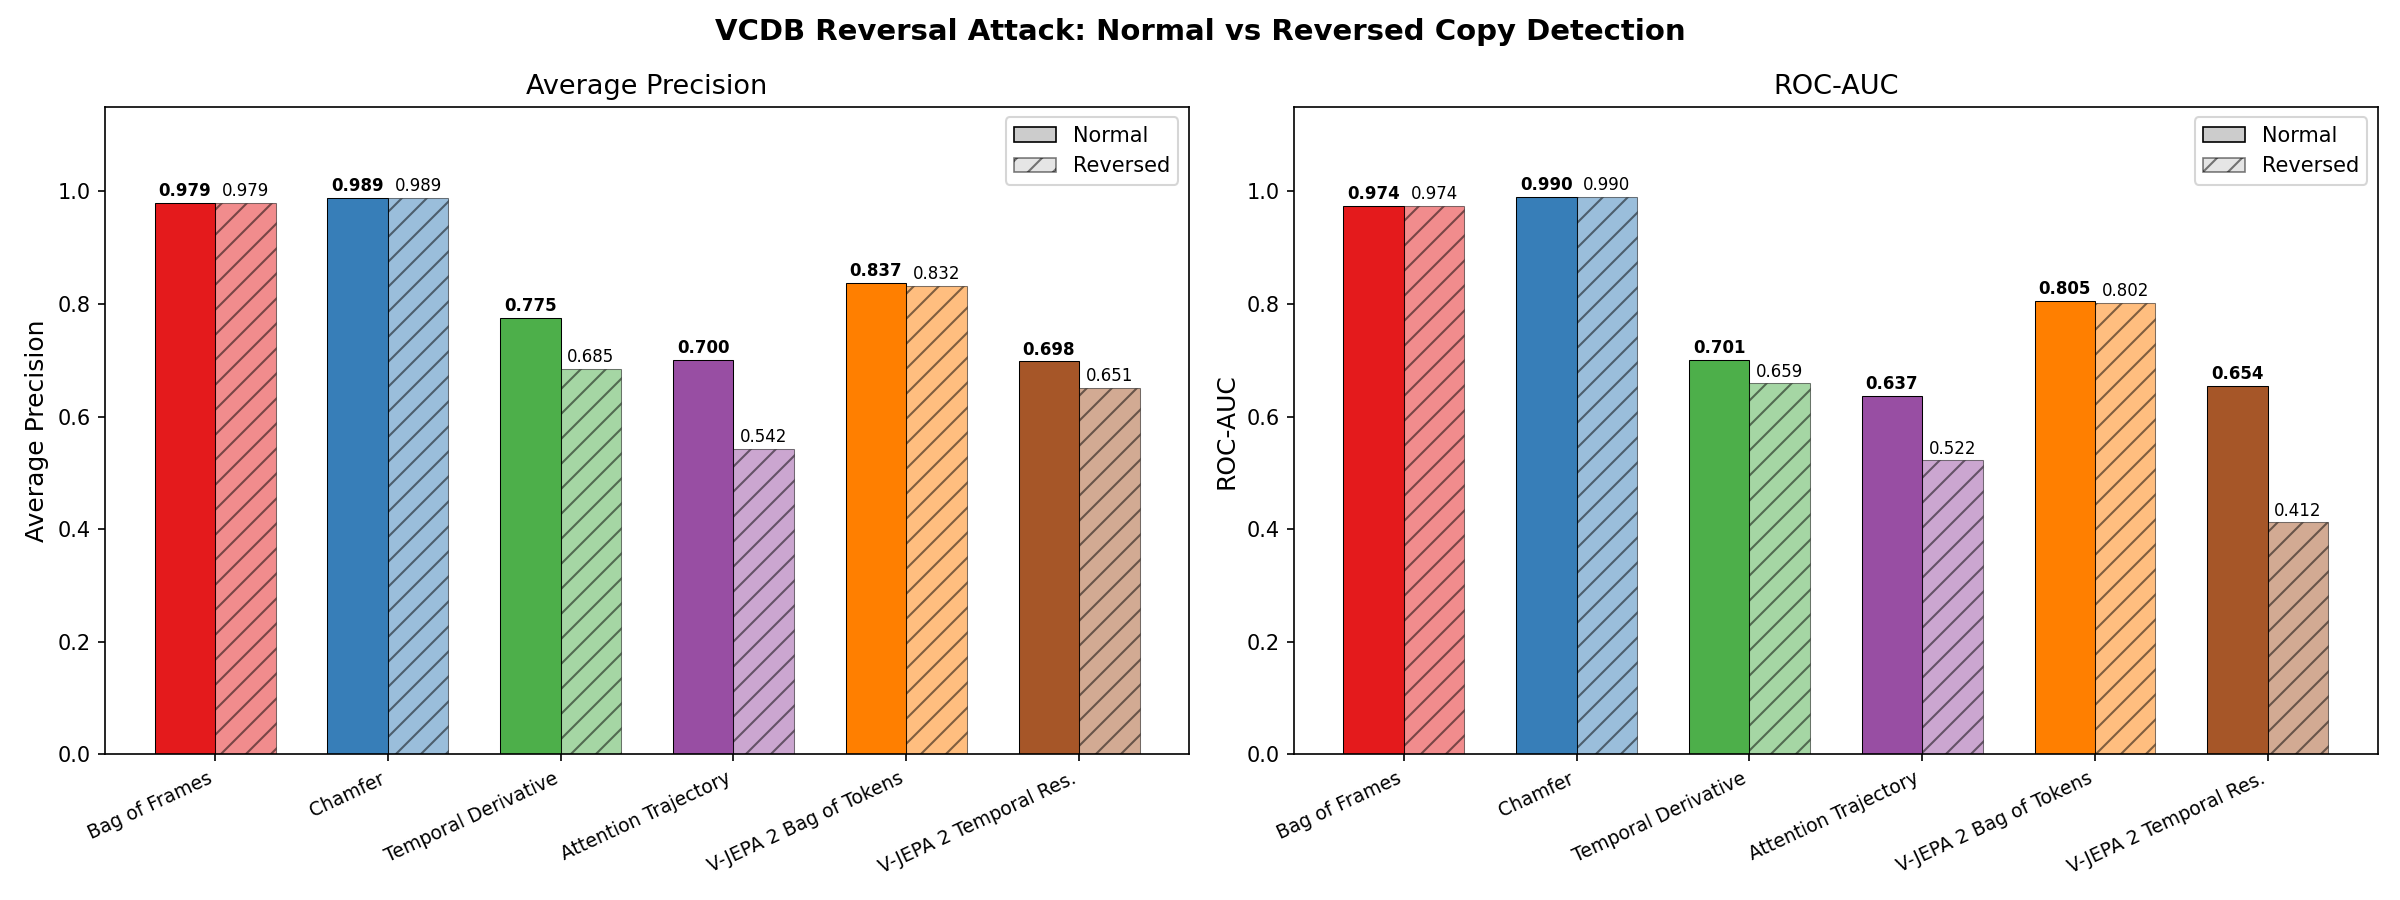
\includegraphics[width=0.9\textwidth]{../figures/vcdb_reversal_attack.png}
    \caption{VCDB Reversal Attack (528 videos, 5{,}585 positive pairs). Order-invariant methods (BoF, Chamfer) maintain identical AP/AUC under reversal. Only sequence-aware methods (Attention Trajectory) register the structural tampering via an AP drop.}
    \label{fig:reversal_attack}
\end{figure}

\begin{table}[ht]
\centering
\caption{VCDB Reversal Attack: 5{,}585 positive pairs (AP drop indicates detection of evasion).}
\begin{tabular}{lccc}
\toprule
\textbf{Method} & \textbf{Normal AP} & \textbf{Reversed AP} & \textbf{AP $\Delta$} \\
\midrule
Chamfer (DINOv3) & 0.989 & 0.989 & \textbf{-0.000} (Invariant) \\
BoF (DINOv3) & 0.979 & 0.979 & \textbf{-0.000} (Invariant) \\
BoT (V-JEPA 2) & 0.838 & 0.832 & -0.006 \\
\textbf{Attention Trajectory (DINOv3)} & 0.700 & 0.542 & \textbf{-0.158} (Detects) \\
Temporal Residual (V-JEPA 2) & 0.698 & 0.631 & -0.067 \\
\bottomrule
\end{tabular}
\end{table}

BoF and Chamfer yield exactly zero AP delta under reversal. Only attention trajectory DTW clearly flags the reversed copy ($\Delta = -0.158$); temporal residual also registers a drop ($\Delta = -0.067$). To quantify temporal sensitivity beyond this binary test, we apply chunk-shuffle scrambling at increasing granularity ($K \in \{1, \ldots, 16\}$) across VCDB.

\begin{figure}[ht]
    \centering
    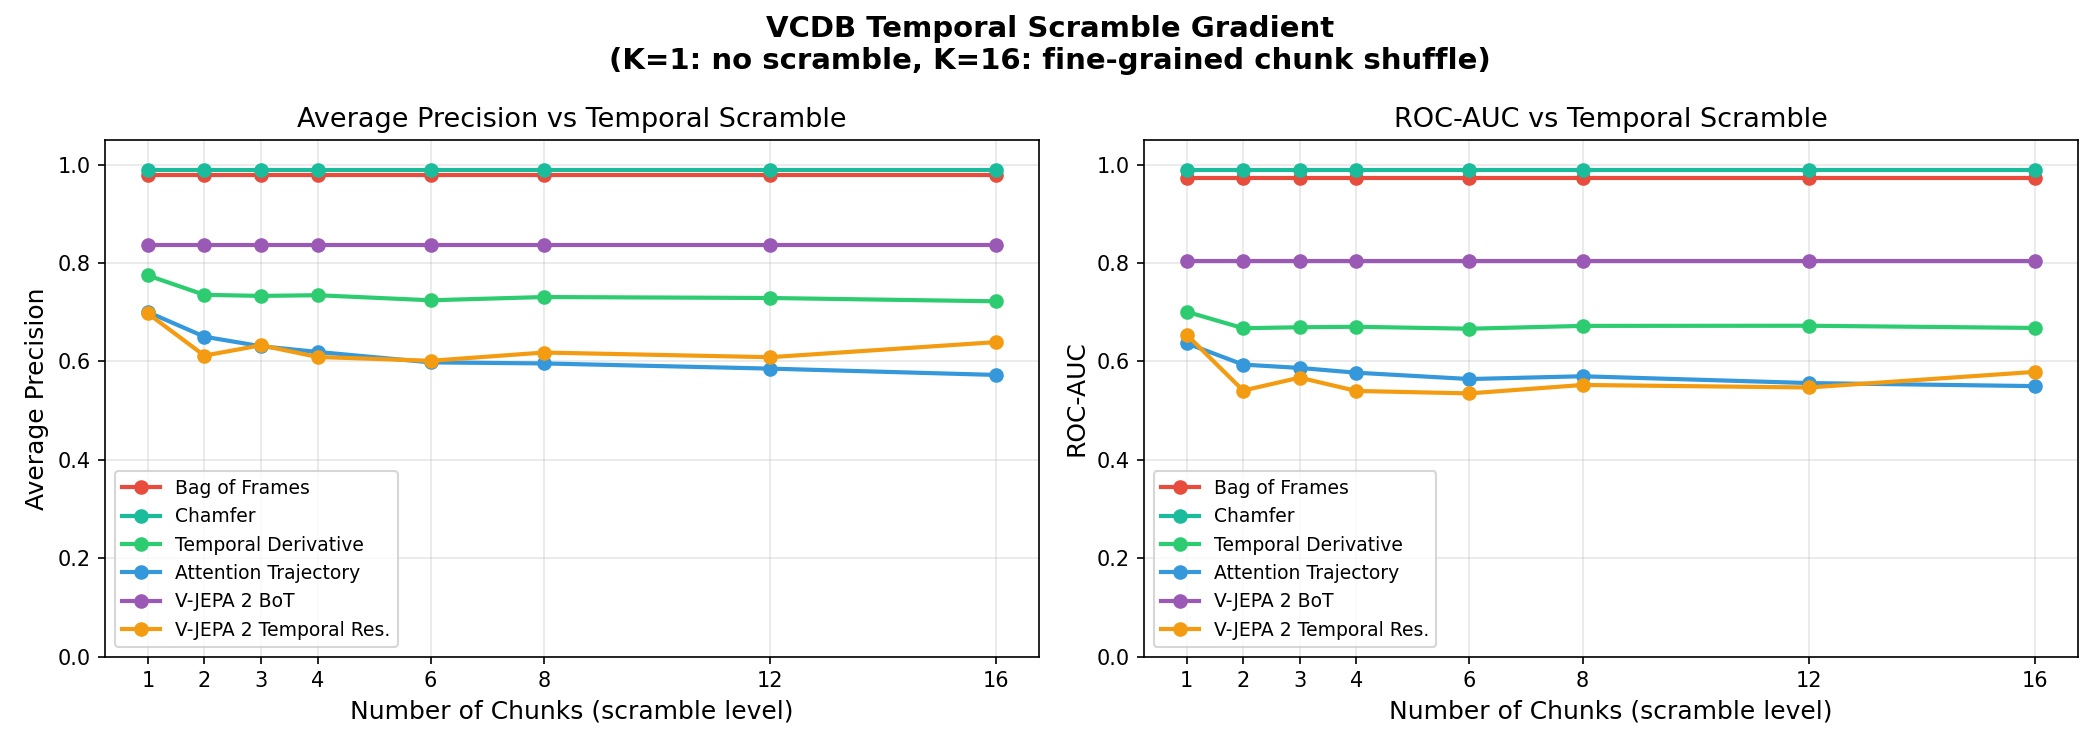
\includegraphics[width=0.9\textwidth]{../figures/vcdb_scramble_gradient.png}
    \caption{Temporal Scramble Gradient on VCDB (527 of 528 videos; one decode failure; 5{,}585 positive pairs). Order-invariant methods (BoF, Chamfer, V-JEPA~2 BoT) maintain constant AP regardless of scramble severity. Sequence-aware methods show overall degradation, with attention trajectories declining most steeply ($-18.3\%$ relative); V-JEPA~2 residual exhibits non-monotonic variation, possibly due to boundary effects at chunk boundaries (Appendix~\ref{sec:scramble_data}).}
    \label{fig:scramble_gradient}
\end{figure}

The scramble gradient separates method classes (Figure~\ref{fig:scramble_gradient}; full table in Appendix~\ref{sec:scramble_data}): order-invariant methods show no sensitivity, while attention trajectories degrade most ($-18.3\%$ relative from $K\!=\!1$ to $K\!=\!16$), as expected since gaze paths are the most temporally structured signal.

\subsection{High-Overlap Motion: Honda HDD \& nuScenes}

To isolate motion from appearance, we clustered 128 Honda HDD~\cite{honda_hdd} driving sessions by RTK GPS, extracting 1{,}687 maneuvers at 50 mixed-direction intersections where BoF similarity averages $0.63 \pm 0.18$ regardless of turn direction (Appendix~\ref{sec:hdd_qualitative}). The full dataset is passage-dominated (${\sim}66\%$), so AP is partially inflated by easier passing-vs-turn negatives.

\begin{table}[ht]
\centering
\caption{Honda HDD Maneuver Discrimination: 1{,}687 maneuvers across 128 sessions, 50 mixed-direction intersection clusters (same vs.\ different turn at same intersection).}
\begin{tabular}{lcc}
\toprule
\textbf{Method} & \textbf{AP} & \textbf{AUC} \\
\midrule
DINOv3 Temporal Deriv. & 0.498 & 0.526 \\
DINOv3 Attn.\ Trajectory & 0.507 & 0.541 \\
DINOv3 BoF & 0.530 & 0.542 \\
DINOv3 Chamfer & 0.559 & 0.577 \\
ViCLIP (InternVid-10M) & 0.542 & 0.549 \\
TARA (chiral, cosine) & 0.547 & 0.600 \\
PL-Stitch BoF & 0.478 & 0.512 \\
PL-Stitch Chamfer & 0.498 & 0.547 \\
PL-Stitch Temporal Deriv. & 0.492 & 0.523 \\
PL-Stitch DTW (raw emb.) & 0.540 & 0.548 \\
\midrule
V-JEPA 2 BoT & 0.825 & 0.836 \\
V-JEPA 2 Encoder-Seq DTW & 0.942 & 0.935 \\
\textbf{V-JEPA 2 Temporal Residual} & \textbf{0.956} & \textbf{0.952} \\
\bottomrule
\end{tabular}
\end{table}

DINOv3 methods fail (AP $\approx$ 0.50): dashcam attention tracks salient objects identical for both turns. V-JEPA~2 temporal residuals achieve AP\,=\,0.956; a pixel-difference motion proxy rules out a trivial intensity shortcut (Spearman $r = 0.051$; Appendix~\ref{sec:hdd_leakage}), and optical flow (RAFT) achieves only AP\,=\,0.478. Restricting to left-vs-right pairs only yields AP\,=\,0.960 [0.958, 0.963]. To disentangle feature from comparator, we compare encoder patches via DTW: encoder-sequence DTW achieves AP\,=\,0.942, showing that 89\% of the BoT-to-residual gap (0.825 $\to$ 0.956) comes from the comparator (cosine $\to$ DTW). We restrict encoder-sequence DTW to motion tasks (HDD, nuScenes); on VCDB, BoF already achieves AP\,=\,0.989.

Two encoders trained with explicit temporal objectives reinforce the comparator finding. TARA~\cite{tara}, a 7B-parameter MLLM trained with chiral negatives, achieves AP\,=\,0.547 under cosine---indistinguishable from ViCLIP (0.542) despite ${\sim}23\times$ more parameters and temporal-specific training. PL-Stitch~\cite{plstitch} (ViT-Base, Plackett-Luce ranking) supports the same decomposition: BoF yields AP\,=\,0.478, DTW on raw embeddings 0.540---both near chance. PL-Stitch falls below DINOv3 across all four methods (e.g., Chamfer 0.498 vs.\ 0.559); the 86M-parameter encoder lacks capacity regardless of comparator. Yet $s_\text{rev}\!=\!0.006$ under raw DTW confirms that PL-Stitch \emph{does} encode frame order---the features are not discriminative enough for maneuver retrieval.

\begin{figure}[ht]
    \centering
    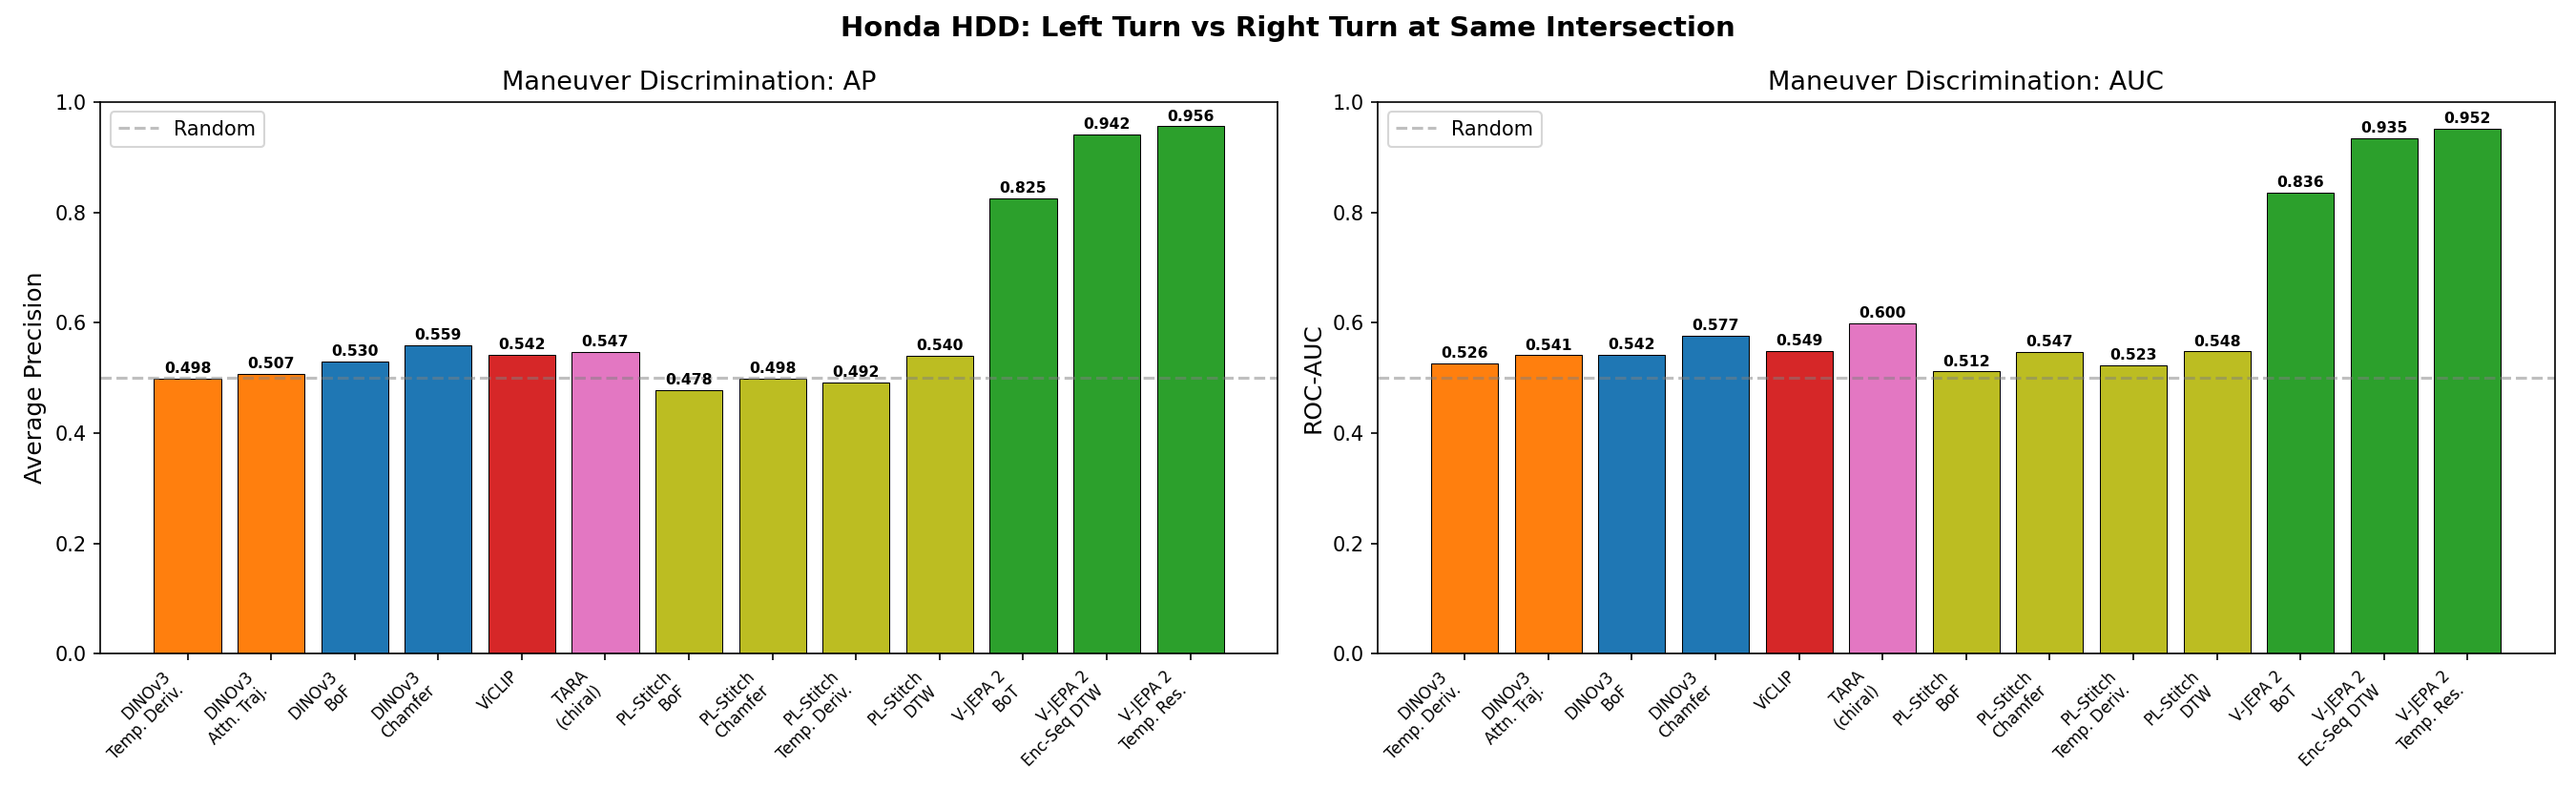
\includegraphics[width=0.9\textwidth]{../figures/hdd_maneuver_discrimination.png}
    \caption{Honda HDD maneuver discrimination (1{,}687 maneuvers, 128 sessions). V-JEPA~2 temporal residuals achieve near-perfect separation (AP\,=\,0.956) while DINOv3 methods remain at chance.}
    \label{fig:hdd_maneuver}
\end{figure}

\subsubsection{Sampling Density: Context Window Sweep}
\label{sec:context_sweep}

We fix the backbone and pair set on HDD and sweep clip duration via \texttt{context\_sec} $\in \{1.0, \ldots, 8.0\}$ while always extracting 64 unique frames ($\text{fps}_\text{eff} = 64 / d$), avoiding the padding confound of the FPS downsample experiment (Appendix~\ref{sec:fps_invariance}).

\begin{figure}[ht]
    \centering
    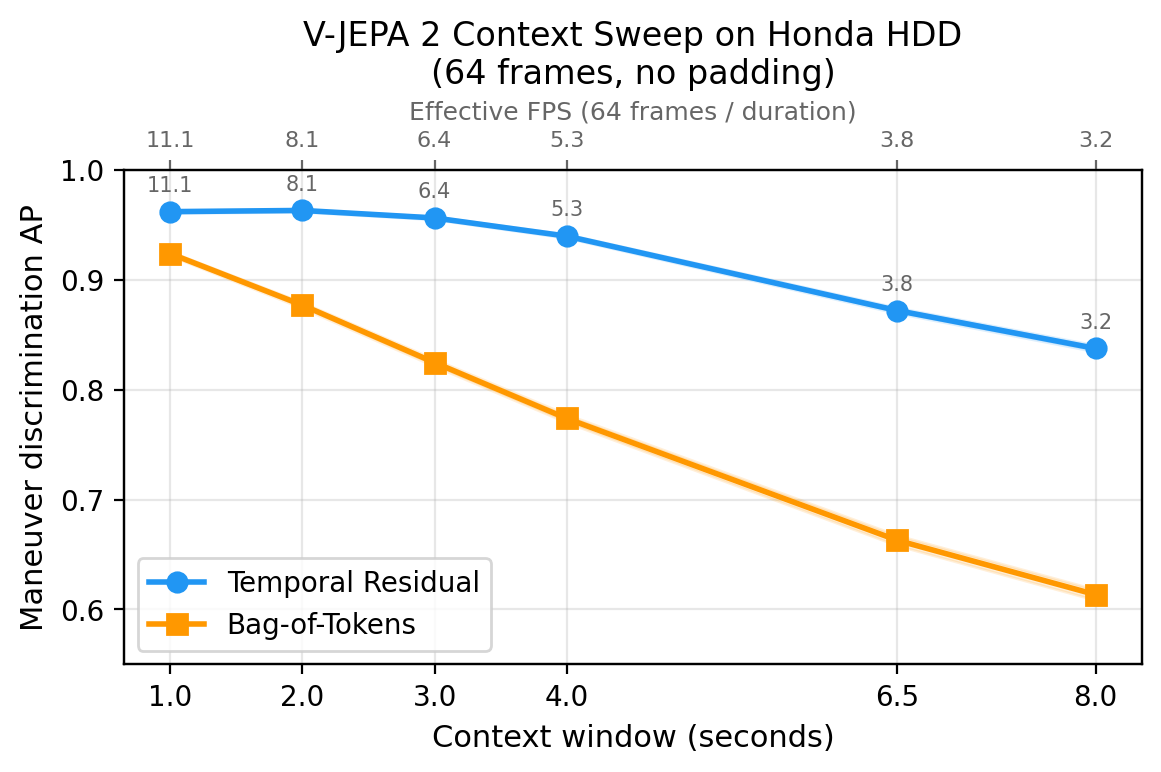
\includegraphics[width=0.9\textwidth]{../figures/hdd_context_sweep.png}
    \caption{V-JEPA~2 context sweep on Honda HDD (1{,}687 maneuvers, 128 sessions). Temporal residual degrades more slowly than BoT; the gap grows from $+0.038$ at 1\,s to $+0.224$ at 8\,s (full table in Appendix~\ref{sec:context_sweep_table}).}
    \label{fig:context_sweep}
\end{figure}

\subsubsection{Cross-Dataset Validation: nuScenes}
\label{sec:nuscenes}

To test whether the method ranking transfers to a different platform, we evaluate on nuScenes~\cite{nuscenes}, a different vehicle, camera, and environment. Turn labels come from CAN bus telemetry; intersections are clustered via DBSCAN ($\epsilon\!=\!30$m), yielding 264 segments across 50 mixed-direction clusters (950 pairs).

The method ranking is directionally consistent (Table~\ref{tab:summary}): V-JEPA~2 encoder-sequence DTW achieves AP\,=\,0.867, surpassing the temporal residual (0.815) and BoT (0.791), with all DINOv3 methods at $\leq$0.623. Encoder-sequence DTW (raw encoder patches under DTW, without the residual transform) outperforms the temporal residual, confirming the comparator as the primary driver---consistent with HDD. Bootstrap CIs show marginal overlap ([0.842,\,0.890] vs.\ [0.785,\,0.844]; Appendix~\ref{sec:bootstrap_cis}). The residual helps on HDD (0.956 vs.\ 0.942) but not nuScenes (0.815 vs.\ 0.867), likely because nuScenes' native 2\,Hz yields sparser temporal gradients where prediction errors add noise. nuScenes at native 2\,Hz outperforms HDD subsampled to 2\,FPS with repeat-padding (AP\,=\,0.636), suggesting native keyframes preserve more temporal signal (Figure~\ref{fig:nuscenes_maneuver}, Appendix~\ref{sec:nuscenes_figure}).

\subsection{VLM Temporal Blindness (EPIC-Kitchens)}

Prior work documents temporal blindness in Video-LLMs for generative QA~\cite{tomato,temporalbench,tempcompass,infact,videozerobench}. We extend this to \emph{retrieval embeddings}, probing where temporal signal dies. We evaluate three VLMs on 500 EPIC-Kitchens-100~\cite{epickitchens} sequences: Qwen3-VL-8B, Gemma-4-31B, and LLaVA-Video-7B.

\subsubsection{Generative Probes}
\label{sec:vlm_generative}

Each model received identical frames with three semantically equivalent prompts asking to classify temporal direction.

\begin{table}[ht]
\centering
\caption{VLM forward/reverse classification on EPIC-Kitchens (500 sequences for open-weight models, 200 for API models). All at or near chance. $\pm$ values are standard deviation across prompts.}
\begin{tabular}{lcccc}
\toprule
\textbf{Model} & \textbf{Prompt 0} & \textbf{Prompt 1} & \textbf{Prompt 2} & \textbf{Mean Bal.\ Acc.} \\
\midrule
Qwen3-VL-8B & 0.517 & 0.502 & 0.504 & $0.508 \pm 0.007$ \\
Gemma-4-31B & 0.549 & 0.528 & 0.535 & $0.538 \pm 0.009$ \\
LLaVA-Video-7B & 0.503 & 0.501 & 0.505 & $0.503 \pm 0.002$ \\
\midrule
Claude 4.6 Opus & 0.490 & 0.590 & 0.555 & $0.545 \pm 0.055$ \\
Gemini 3.1 Pro & 0.585 & 0.608 & 0.603 & $0.599 \pm 0.010$ \\
\bottomrule
\end{tabular}
\end{table}

All five models perform at or near chance; Gemini~3.1 Pro~\cite{gemini31pro} (a reasoning model) reaches $0.599 \pm 0.010$---marginally above chance but far from reliable. Answers are driven by prompt phrasing, not temporal direction (Appendix~\ref{sec:integrity_probe} and~\ref{sec:prompt_details}).

\subsubsection{Embedding Probes: Where Temporal Signal Dies}
\label{sec:vlm_embedding}

VLMs \emph{output} answers carrying no temporal information. We probe whether temporal signal persists in internal representations but is discarded.

\begin{table}[ht]
\centering
\caption{Order sensitivity ($s_\text{rev}$) across the VLM pipeline on EPIC-Kitchens (500 sequences) with bootstrap 95\% CIs where available. $s_\text{rev} \approx 1.0$ = order-invariant; lower = more order-sensitive. DINOv3 structural fingerprints shown for reference.$^*$}
\label{tab:vlm_embedding}
\begin{tabular}{lcc}
\toprule
\textbf{Method} & $s_\text{rev}$$\downarrow$ \textbf{[95\% CI]} & \textbf{Bal.\ Acc.$\uparrow$} \\
\midrule
\multicolumn{3}{l}{\emph{DINOv3 structural fingerprints (reference)}} \\
\quad BoF & 1.000 & N/A \\
\quad Chamfer & 0.9999 & N/A \\
\quad Temporal Derivative & 0.500 [0.499, 0.500] & 1.000 \\
\quad Attention Trajectory & 0.192 [0.187, 0.197] & 1.000 \\
\midrule
\multicolumn{3}{l}{\emph{V-JEPA 2}} \\
\quad BoT & 0.984 & 0.500 \\
\quad Temporal Residual & 0.699 & 0.778 \\
\midrule
\multicolumn{3}{l}{\emph{VLM vision towers (pooled)}} \\
\quad Gemma-4 (SigLIP) & 1.000$^\dagger$ & N/A \\
\quad LLaVA (CLIP) & 1.000$^\dagger$ & N/A \\
\midrule
\multicolumn{3}{l}{\emph{VLM vision sequence (per-frame DTW)}} \\
\quad Gemma-4 (SigLIP) & 0.492 [0.491, 0.493] & 1.000 \\
\quad LLaVA (CLIP) & 0.495 [0.495, 0.496] & 1.000 \\
\midrule
\multicolumn{3}{l}{\emph{VLM LLM hidden state}} \\
\quad Gemma-4 (Gemma) & 1.000 [1.000, 1.000] & N/A \\
\quad LLaVA (Qwen2) & 0.998 [0.998, 0.999] & N/A \\
\quad Qwen3-VL (Qwen3) & 0.998 [0.998, 0.999] & N/A \\
\bottomrule
\end{tabular}
\begin{flushleft}
\small $^*$DINOv3 300M params, CLIP (ViT-L) 304M, SigLIP (SO-400M) 400M. Order-invariance follows from the aggregation operator (Observation~\ref{obs:pooling}), not model capacity. $^\dagger$Raw values 1.001--1.002 from f32 precision; clamped to 1.000. Qwen3-VL vision probes are omitted from this table because its ViT uses dynamic-resolution spatial grids with 3D temporal--spatial merging, preventing clean per-frame token grouping for the detailed $s_\text{rev}$ analysis; approximate pooled and sequence results appear in Table~\ref{tab:summary}. The LLM hidden-state probe (below) is unaffected.
\end{flushleft}
\end{table}

\textbf{Order signal is recoverable from per-frame features but erased by pooling.} Pooled VLM vision embeddings are perfectly order-invariant ($s_\text{rev} \approx 1.0$), but retaining per-frame tokens and comparing via temporal derivative DTW achieves perfect forward/reverse separation (balanced accuracy\,=\,1.000). \textbf{Caveat:} this follows from the mathematical structure of temporal derivatives under DTW (reversed derivatives are negated), not learned temporal understanding. The pattern holds for both CLIP and SigLIP~\cite{weller2025limits}. Qwen3-VL's pooled vision embeddings underperform sharply (VCDB AP\,=\,0.491 vs.\ 0.915--0.926 for LLaVA/Gemma), likely because its dynamic-resolution spatial grids with 3D temporal--spatial merging entangle frame identity with spatial position, degrading the pooled representation for retrieval.

The LLM backbone does not surface this signal under any pooled readout ($s_\text{rev} = 0.998$--$1.000$ across all layers; Appendix~\ref{sec:layer_ablation}). Neither logistic regression nor 2-layer MLP probes on per-position LLM hidden states recover temporal order above chance (GroupKFold CV, fwd/rev pairs kept together, seven pooling strategies; best: 0.560; all 126 configurations within chance range; Appendix~\ref{sec:linear_probe}). Yet per-position hidden states \emph{do} retain order signal under full-sequence DTW (Appendix~\ref{sec:vision_token_probe}). Symmetric aggregation, not the LLM backbone itself, is the bottleneck.

\subsection{Cross-Method Summary}

Table~\ref{tab:summary} consolidates results across all benchmarks; no single method dominates every paradigm.

\begin{table}[ht]
\centering
\caption{All methods across all tasks (VCDB: 5{,}585 pairs; HDD: 1{,}687 maneuvers; nuScenes: 950 pairs; EPIC: 500 sequences). Nymeria and MUVR scene-matching results replicate the VCDB finding (BoF dominates) and are in Appendix~\ref{sec:scene_matching}. AP values are point estimates; 95\% bootstrap CIs (2{,}000 resamples, percentile method) are in Appendix~\ref{sec:bootstrap_cis}.}
\label{tab:summary}
\resizebox{\textwidth}{!}{%
\begin{tabular}{lccccc}
\toprule
\textbf{Method} & \textbf{VCDB (AP$\uparrow$)} & \textbf{HDD (AP$\uparrow$)} & \textbf{nuScenes (AP$\uparrow$)} & \textbf{EPIC $s_\text{rev}$$\downarrow$} & \textbf{EPIC Bal.\ Acc.$\uparrow$} \\
\midrule
DINOv3 BoF & 0.979 & 0.530 & 0.613 & 1.000 & N/A \\
DINOv3 Chamfer & \textbf{0.989} & 0.559 & 0.612 & 0.9999 & N/A \\
DINOv3 Temporal Deriv. & 0.775 & 0.498 & 0.623 & 0.500 & \textbf{1.000} \\
DINOv3 Attn.\ Trajectory & 0.700 & 0.507 & 0.584 & \textbf{0.192} & \textbf{1.000} \\
V-JEPA 2 BoT & 0.838 & 0.825 & 0.791 & 0.984 & 0.500 \\
V-JEPA 2 Encoder-Seq DTW & --- & 0.942 & \textbf{0.867} & --- & --- \\
V-JEPA 2 Temporal Res. & 0.698 & \textbf{0.956} & 0.815 & 0.699 & 0.778 \\
ViCLIP (InternVid-10M) & 0.907 & 0.542 & 0.618 & 0.996 & N/A \\
TARA (chiral, cosine) & --- & 0.547 & --- & 0.955 & N/A \\
PL-Stitch BoF & --- & 0.478 & --- & 1.000 & N/A \\
PL-Stitch DTW (raw emb.) & --- & 0.540 & --- & 0.006 & N/A \\
X-CLIP (16-frame) & 0.960 & --- & --- & 0.980 & N/A \\
Optical Flow (RAFT) DTW & --- & 0.478 & --- & --- & --- \\
\midrule
Qwen3-VL-8B (gen.) & 0.519$^\ddagger$ & 0.531$^\ddagger$ & 0.487$^\ddagger$ & N/A & 0.508 \\
Gemma-4-31B (gen.) & 0.559$^\ddagger$ & 0.510$^\ddagger$ & 0.529$^\ddagger$ & N/A & 0.538 \\
LLaVA-Video-7B (gen.) & 0.521$^\ddagger$ & 0.500$^\ddagger$ & 0.507$^\ddagger$ & N/A & 0.503 \\
Claude 4.6 Opus (gen.) & ---$^\ddagger$ & ---$^\ddagger$ & ---$^\ddagger$ & N/A & 0.545 \\
Gemini 3.1 Pro (gen.) & ---$^\ddagger$ & ---$^\ddagger$ & ---$^\ddagger$ & N/A & 0.599 \\
\midrule
Gemma-4 vision pooled (SigLIP) & 0.926 & 0.521 & 0.662 & 1.000$^\dagger$ & N/A \\
LLaVA vision pooled (CLIP) & 0.915 & 0.514 & 0.624 & 1.000$^\dagger$ & N/A \\
Qwen3 vision pooled (SigLIP) & 0.491 & 0.421 & 0.464 & 0.998$^\dagger$ & N/A \\
Gemma-4 vision seq (SigLIP) & 0.632 & 0.553 & 0.469 & 0.492 & \textbf{1.000} \\
LLaVA vision seq (CLIP) & 0.637 & 0.545 & 0.470 & 0.495 & \textbf{1.000} \\
Qwen3 vision seq (SigLIP) & 0.610 & 0.468 & 0.517 & 0.542 & \textbf{1.000} \\
VLM LLM hidden state (Gemma-4) & 0.838 & 0.472 & 0.569 & $\geq$0.998 & N/A \\
VLM LLM hidden state (LLaVA) & 0.907 & 0.512 & 0.652 & $\geq$0.998 & N/A \\
VLM LLM hidden state (Qwen3) & 0.916 & 0.518 & 0.630 & $\geq$0.998 & N/A \\
\bottomrule
\end{tabular}
}
\begin{flushleft}
\small $^\dagger$Pooled representations are order-invariant by construction. --- = not evaluated.
$^\ddagger$Generative balanced accuracy (forward/reverse classification); not retrieval AP. All VLMs perform at or near chance. $s_\text{rev}$ is N/A for generative models. VCDB AP depends on negative seed ($\pm$0.06; Appendix~\ref{sec:neg_sampling}). Claude and Gemini evaluated on EPIC-Kitchens only (200 sequences each via API).
\end{flushleft}
\end{table}

\section{Related Work}
\label{sec:related_work}

\textbf{Video copy detection.} Standard benchmarks (ISC~\cite{douze2021isc}, VSC~\cite{pizzi2023vsc}, VCSL~\cite{he2022vcsl}) and descriptors (SSCD~\cite{pizzi2022sscd}, ViSiL~\cite{kordopatis2019visil}, DnS~\cite{kordopatis2022dns}, S2VS~\cite{s2vs}) provide per-frame features with learned aggregation. Wang et al.~\cite{wang2023duallevel} win the Meta VSC challenge; subsequent analysis~\cite{fojcik2025} exposes temporal-attack vulnerability. Explicit temporal alignment (VSAL~\cite{han2021vsal}, TransVCL~\cite{he2023transvcl}) shows order matters for copy localization. We diagnose \emph{when} temporal structure helps versus hurts.

\textbf{Temporal sensitivity in video models.} Lei et al.~\cite{lei2022singleframe} established the static-bias problem. Subsequent work diagnoses this in generative VLM QA~\cite{tempcompass,bagad2023testtime,temporalbench,vbenchcomp,tomato,videozerobench,infact}. Arrow-of-time diagnostics~\cite{aot,arrowrl} and further studies~\cite{timeblindness,timeblind,vitatecs,reveal,weavetime} show the failure is structural; PL-Stitch~\cite{plstitch} and ArrowGEV~\cite{arrowgev} propose training-time fixes. MASH-VLM~\cite{mashvlm} identifies RoPE positional bias; TIPSv2~\cite{tipsv2} shows scaling worsens alignment. We differ in \emph{domain} (retrieval) and \emph{granularity} (localizing failure to aggregation via scramble gradients and feature-vs-comparator decomposition). TGPO~\cite{tgpo} uses binary ordered-vs-shuffled RL reward; our scramble gradient extends this to a continuous $K$-parameterized diagnostic. TARA~\cite{tara} introduces chiral negatives for training; we use reversal as a diagnostic probe.

\textbf{Video prediction for temporal understanding.} V-JEPA~2~\cite{vjepa2} learns spatiotemporal representations via masked prediction; Drive-JEPA~\cite{drivejepa} applies these to driving; TWLV-I~\cite{twlvi} evaluates appearance vs.\ motion across video foundation models. Li et al.~\cite{temporaltransfer} show temporal information is encoded but standard pipelines fail to surface it, matching our finding. Co-Settle~\cite{cosettle} formalizes temporal consistency vs.\ semantic separability; our sensitivity--invariance analysis maps a related trade-off.

\textbf{Temporal alignment for retrieval.} DTW~\cite{sakoe1978dtw} remains standard; extensions include differentiable DTW~\cite{ddtw} and Drop-DTW~\cite{dropdtw}. At $T \approx 30$ frames, each comparison takes ${\sim}1$\,ms; top-100 reranking after FAISS~\cite{faiss} adds ${\sim}100$\,ms. We use DTW as a diagnostic tool; Weller et al.~\cite{weller2025limits} provide theoretical justification for multi-vector approaches.

\section{Discussion}
\label{sec:discussion}

No single method dominates. \textbf{(i)~Scene matching} (VCDB, Nymeria, MUVR): BoF is optimal; temporal methods add noise (Appendix~\ref{sec:scene_matching}). \textbf{(ii)~Motion dynamics} (Honda HDD, nuScenes): requires spatiotemporal processing (V-JEPA~2); per-frame methods and VLM vision towers all fail (AP\,$\leq$\,0.56), with the residual advantage growing under sparser sampling (Section~\ref{sec:context_sweep}); 89\% of the BoT-to-residual gap comes from the comparator (cosine$\to$DTW) on HDD, and on nuScenes the encoder-sequence DTW alone surpasses the temporal residual (AP\,=\,0.867 vs.\ 0.815), confirming that the comparator is the primary driver. Even video-native ViCLIP~\cite{viclip} ($s_\text{rev}\!=\!0.996$, HDD AP\,=\,0.542) and X-CLIP~\cite{xclip} ($s_\text{rev}\!=\!0.980$) do not escape the blind spot, though ViCLIP's 8-frame input partially confounds this (see Limitations). Models trained with explicit temporal objectives fare no better under symmetric comparators: TARA~\cite{tara} (chiral negatives, HDD AP\,=\,0.547) and PL-Stitch~\cite{plstitch} BoF (temporal ranking, AP\,=\,0.478) fail under cosine similarity; PL-Stitch also fails under DTW (AP\,=\,0.540), falling below DINOv3 Chamfer (0.559)---the 86M encoder lacks capacity, though $s_\text{rev}\!=\!0.006$ under raw DTW confirms it encodes frame order. \textbf{(iii)~Temporal manipulation} (reversal, scrambling): requires explicit sequence tracking; implicit 3D models~\cite{3dcsl}, frame-sampling defenses~\cite{fojcik2025}, and Video-LLMs all remain order-invariant~\cite{plstitch, aot}; TARA's chiral training lowers $s_\text{rev}$ to 0.955 (vs.\ ViCLIP's 0.996)---improved but insufficient for retrieval; a reasoning model (Gemini~3.1 Pro) reaches $0.599$ (vs.\ ${\leq}0.545$ for non-reasoning VLMs) but remains far from reliable. Per-frame features separate forward/reverse under DTW (by construction), but pooling erases it; LLM hidden states stay order-invariant across all layers.

\begin{figure}[ht]
    \centering
    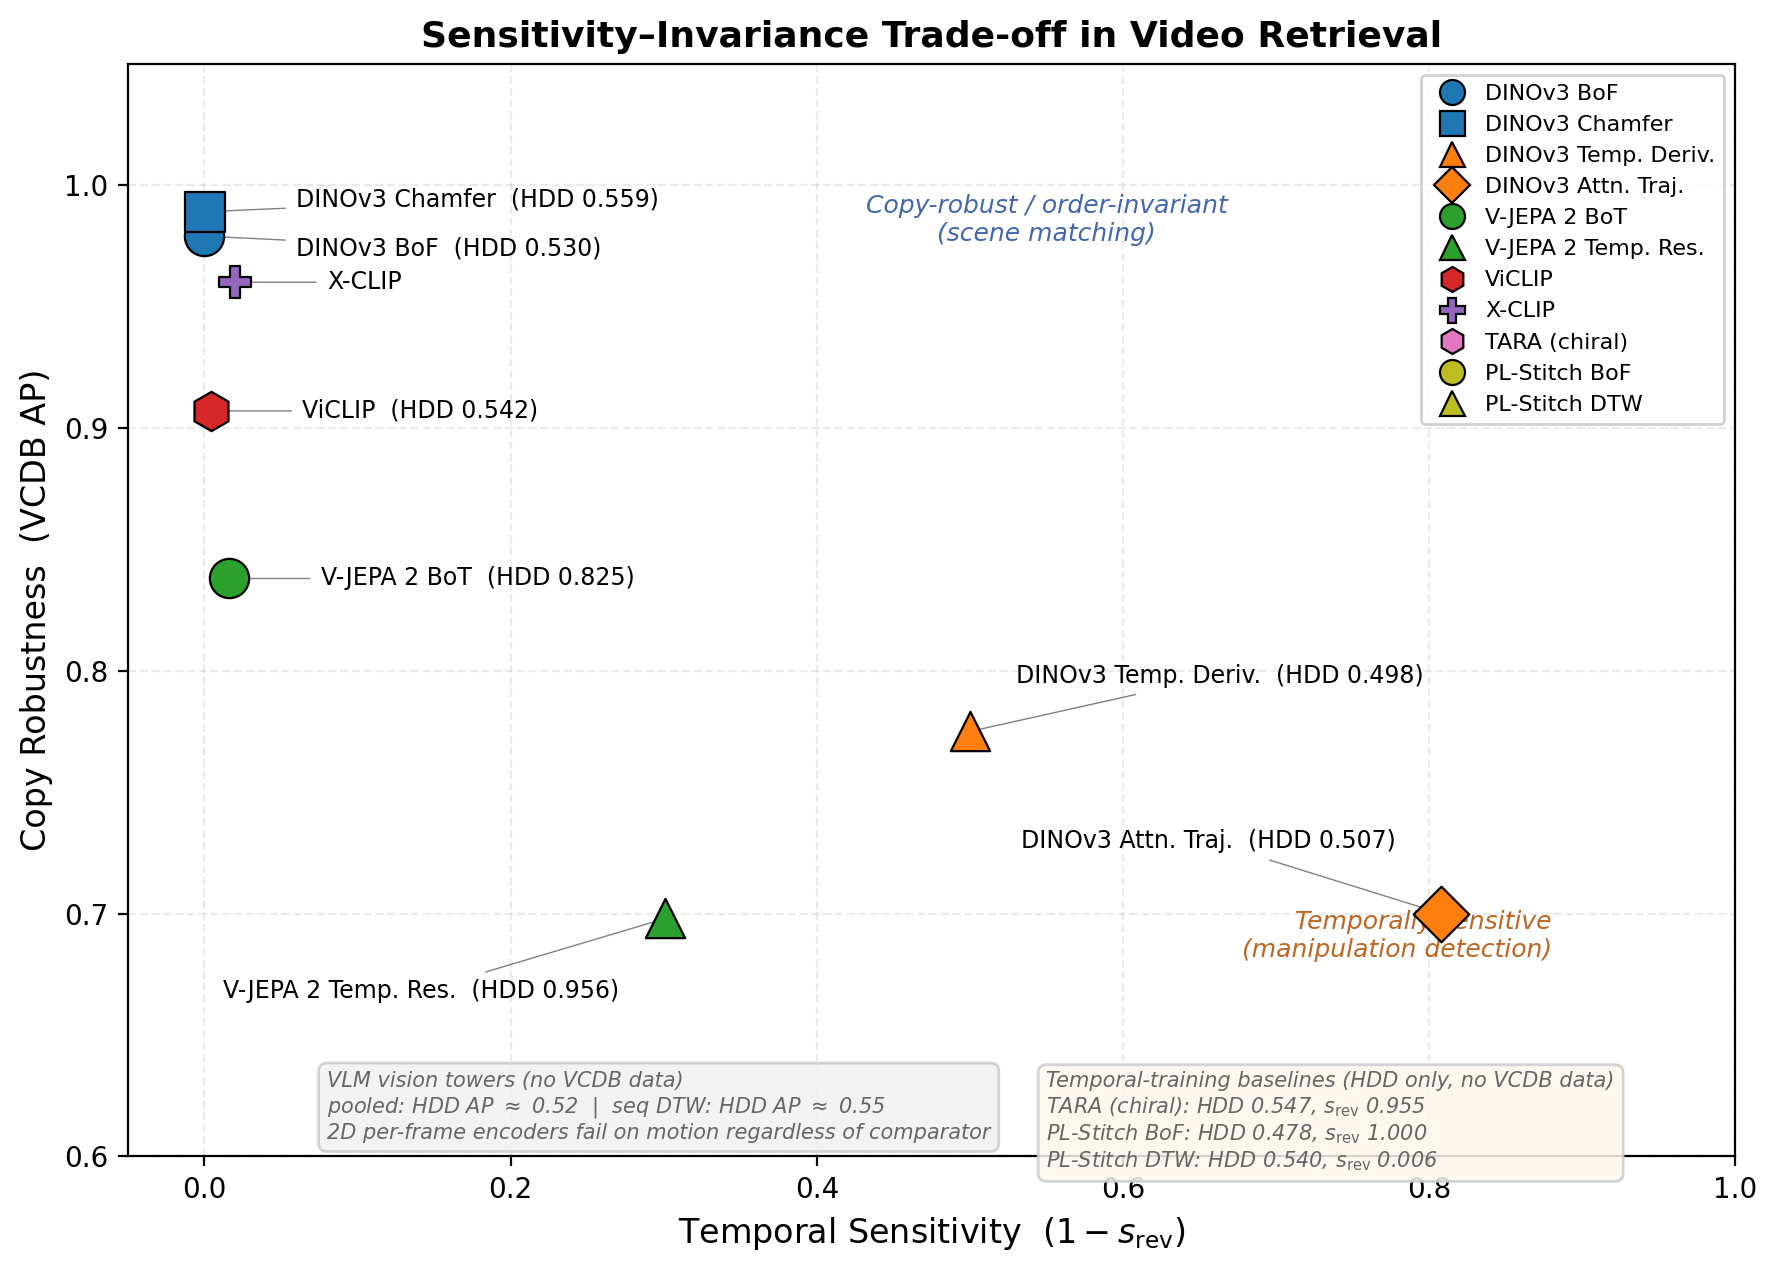
\includegraphics[width=0.6\textwidth]{../figures/sensitivity_invariance_tradeoff.png}
    \caption{Sensitivity--invariance trade-off: temporal sensitivity ($1 - s_\text{rev}$, EPIC) vs.\ copy robustness (VCDB AP). No method occupies the upper-right quadrant. Note: pooled and sequence $s_\text{rev}$ use different similarity functions (cosine vs.\ DTW) and are not directly comparable on this axis; see Eq.~\eqref{eq:srev}.}
    \label{fig:sensitivity_invariance}
\end{figure}

\textbf{Limitations.} All evaluations use pairwise similarity; DTW is not indexable ($O(T^2)$); probes train on 400 samples ($p \gg n$); ViCLIP's 8-frame input confounds its comparison with 64-frame V-JEPA~2 (Section~\ref{sec:context_sweep} provides a partial control).

\textbf{Practitioner recommendations.} (1)~Test your pipeline with the scramble gradient at $K \in \{1, 4, 16\}$ using \textsc{TemporalDiag} (\texttt{temporal-diag report}): if AP is flat across $K$, the system is temporally blind. (2)~For copy detection, BoF is optimal; adding temporal methods hurts. (3)~For motion-sensitive retrieval, a two-stage pipeline (BoF pre-filter $\to$ DTW rerank on top-$k$) is practical at ${\sim}100$\,ms overhead per query (Appendix~\ref{sec:computational_costs}).

\section{Conclusion}

Across six benchmarks, semantic pooling, trajectory tracking, and spatiotemporal residuals each dominate a distinct retrieval regime; across all methods we evaluate, no single approach spans both copy detection and motion retrieval (Figure~\ref{fig:sensitivity_invariance}). The temporal scramble gradient cleanly separates method classes. The feature-vs-comparator decomposition places 89\% of the gap in the matching function on HDD; on nuScenes, the comparator alone (encoder-sequence DTW) surpasses the residual transform entirely (AP\,=\,0.867 vs.\ 0.815). Encoders trained with temporal objectives---TARA~\cite{tara} (chiral negatives, AP\,=\,0.547) and PL-Stitch~\cite{plstitch} (temporal ranking, AP\,=\,0.540 under DTW)---also fail on HDD, confirming that the comparator, not the training objective, governs retrieval discrimination. VLM embedding probes confirm that pooling erases order information present in per-frame encoders (126 probe configurations at chance). Efficient order-sensitive comparators remain the key open problem.\footnote{%
\ifdefined\neuripssubmission
Code and data: included in supplementary material. All datasets and model weights are publicly available; see \texttt{REPRODUCIBILITY.md}.%
\else
Code: \url{https://github.com/mkatindustries/video-temporal-diagnostics}. All datasets and model weights are publicly available; see \texttt{REPRODUCIBILITY.md}.%
\fi
}

\FloatBarrier  % Force all main-body floats before references

\begin{thebibliography}{99}
\bibitem{vjepa2} A.~Bardes et al. V-JEPA~2. \emph{arXiv:2506.09985}, 2025. See also V-JEPA~2.1 (\emph{arXiv:2603.14482}, 2026).
\bibitem{dinov3} O.~Sim\'{e}oni et al. {DINOv3}. \emph{arXiv:2508.10104}, 2025.
\bibitem{vcdb} Y.~Jiang et al. {VCDB}. In \emph{ECCV}, 2014.
\bibitem{honda_hdd} V.~Ramanishka et al. Toward driving scene understanding. In \emph{CVPR}, 2018.
\bibitem{nuscenes} H.~Caesar et al. nuScenes: A multimodal dataset for autonomous driving. In \emph{CVPR}, 2020.
\bibitem{epickitchens} D.~Damen et al. Rescaling egocentric vision: Collection, pipeline and challenges for EPIC-KITCHENS-100. \emph{IJCV}, 2022.
\bibitem{fojcik2025} K.~Fojcik and P.~Syga. Counteracting temporal attacks in video copy detection. \emph{arXiv:2501.11171}, 2025.
\bibitem{3dcsl} R.~Deng et al. {3D-CSL}. \emph{arXiv:2211.05352}, 2022.
\bibitem{plstitch} C.~Che et al. PL-Stitch. \emph{arXiv:2511.17805}, 2025.
\bibitem{arrowgev} H.~Yu et al. ArrowGEV. \emph{arXiv:2601.06559}, 2026.
\bibitem{weavetime} Y.~Zhang et al. WeaveTime. \emph{arXiv:2602.22142}, 2026.
\bibitem{timeblindness} C.~Chowdhury et al. Time Blindness: Comprehensive Analysis of Temporal Failures in Video Language Models. \emph{arXiv:2505.24867}, 2025.
\bibitem{qwen3vl} Qwen Team. Qwen3-VL: A Visual Language Model for Unified Image and Video Understanding. \emph{arXiv:2502.13923}, 2025.
\bibitem{gemma4} Google DeepMind. Gemma~4 Technical Report. \url{https://ai.google.dev/gemma/docs/core/model_card_4}, 2026.
\bibitem{llavavideo} Z.~Liu et al. LLaVA-Video: An All-in-One Video Understanding Model with Unified Visual Representation. \emph{arXiv:2410.02713}, 2024.
\bibitem{aot} D.~Matta et al. AoT-PsyPhyBENCH: Benchmarking VLMs on arrow-of-time and psychophysical tasks. \emph{arXiv:2502.01789}, 2025.
\bibitem{vitatecs} S.~Li et al. VITATECS: A Diagnostic Dataset for Temporal Concept Understanding of Video-Language Models. In \emph{ECCV}, 2024.
\bibitem{muvr} W.~Lin et al. Multi-Modal Untrimmed Video Retrieval. \emph{NeurIPS}, 2025.
\bibitem{semdedup} A.~Abbas et al. SemDeDup: Data-efficient learning at web-scale through semantic deduplication. \emph{arXiv:2303.09540}, 2023.
\bibitem{faiss} J.~Johnson et al. Billion-scale similarity search with GPUs. \emph{IEEE Transactions on Big Data}, 2019.
\bibitem{trajtok} Y.~Li et al. TrajTok: Trajectory Tokenization for Efficient Video Understanding. \emph{arXiv:2602.22779}, 2026.
\bibitem{ddtw} J.~Mensch and M.~Blondel. Differentiable Dynamic Time Warping. \emph{arXiv:2303.10778}, 2023.
\bibitem{douze2021isc} M.~Douze, G.~Tolias, E.~Pizzi et al. The 2021 Image Similarity Dataset and Challenge. In \emph{NeurIPS Competition Track}, 2021.
\bibitem{pizzi2023vsc} E.~Pizzi, G.~Kordopatis-Zilos et al. The 2023 Video Similarity Dataset and Challenge. In \emph{CVPR Workshop}, 2023.
\bibitem{pizzi2022sscd} E.~Pizzi, S.~D.~Roy, S.~N.~Ravindra, P.~Goyal, and M.~Douze. A Self-Supervised Descriptor for Image Copy Detection. In \emph{CVPR}, 2022.
\bibitem{kordopatis2019visil} G.~Kordopatis-Zilos, S.~Papadopoulos, I.~Patras, and I.~Kompatsiaris. ViSiL: Fine-grained Spatio-Temporal Video Similarity Learning. In \emph{ICCV}, 2019.
\bibitem{kordopatis2022dns} G.~Kordopatis-Zilos, C.~Tzelepis, S.~Papadopoulos, I.~Kompatsiaris, and I.~Patras. DnS: Distill-and-Select for Efficient and Accurate Video Indexing and Retrieval. \emph{IJCV}, 2022.
\bibitem{he2022vcsl} S.~He et al. A Large-scale Comprehensive Dataset and Copy-overlap Aware Evaluation Protocol for Segment-level Video Copy Detection. In \emph{CVPR}, 2022.
\bibitem{he2023transvcl} S.~He et al. TransVCL: Attention-enhanced Video Copy Localization Network with Flexible Supervision. In \emph{AAAI}, 2023.
\bibitem{han2021vsal} Z.~Han, X.~He, M.~Tang, and Y.~Lv. Video Similarity and Alignment Learning on Partial Video Copy Detection. In \emph{ACM~MM}, 2021.
\bibitem{sakoe1978dtw} H.~Sakoe and S.~Chiba. Dynamic Programming Algorithm Optimization for Spoken Word Recognition. \emph{IEEE Trans.\ Acoustics, Speech, and Signal Processing}, 26(1):43--49, 1978.
\bibitem{nymeria} Y.~Ma et al. Nymeria: A Massive Collection of Multimodal Egocentric Daily Activity in the Wild. In \emph{CVPR}, 2025.
\bibitem{reveal} T.~V.~Sethuraman et al. Stress Tests REVEAL Fragile Temporal and Visual Grounding in Video-Language Models. \emph{arXiv:2602.11244}, 2026.
\bibitem{timeblind} B.~Li et al. TimeBlind: A Spatio-Temporal Compositionality Benchmark for Video LLMs. \emph{arXiv:2602.00288}, 2026.
\bibitem{tgpo} Z.~Xu et al. Incentivizing Temporal-Awareness in Egocentric Video Understanding Models. \emph{arXiv:2603.27184}, 2026.
\bibitem{cosettle} Y.~Liu et al. From Static to Dynamic: Exploring Self-supervised Image-to-Video Representation Transfer Learning. In \emph{CVPR}, 2026.
\bibitem{tara} P.~Bagad and A.~Zisserman. TARA: Simple and Efficient Time Aware Retrieval Adaptation of MLLMs. \emph{arXiv:2512.13511}, 2025.
\bibitem{drivejepa} L.~Wang et al. Drive-JEPA: Video JEPA Meets Multimodal Trajectory Distillation for End-to-End Driving. \emph{arXiv:2601.22032}, 2026.
\bibitem{weller2025limits} O.~Weller, D.~Fried, A.~Rush, and B.~Van~Durme. When Are Single-Vector Embeddings All You Need? \emph{arXiv:2508.21038}, 2025.
\bibitem{lei2022singleframe} J.~Lei, T.~L.~Berg, and M.~Bansal. Revealing Single Frame Bias for Video-and-Language Learning. \emph{arXiv:2206.03428}, 2022.
\bibitem{bagad2023testtime} P.~Bagad, M.~Tapaswi, and C.~G.~M.~Snoek. Test of Time: Instilling Video-Language Models with a Sense of Time. In \emph{CVPR}, 2023.
\bibitem{tempcompass} Y.~Liu, S.~Li, Y.~Liu et al. TempCompass: Do Video LLMs Really Understand Videos? \emph{arXiv:2403.00476}, 2024.
\bibitem{twlvi} H.~Lee, J.-Y.~Kim, K.~Baek et al. TWLV-I: Analysis and Insights from Holistic Evaluation on Video Foundation Models. \emph{arXiv:2408.11318}, 2024.
\bibitem{temporaltransfer} L.~Li, Y.~Liu, Y.~Yao et al. Temporal Reasoning Transfer from Text to Video. \emph{arXiv:2410.06166}, 2024.
\bibitem{tomato} Z.~Shangguan, C.~Li, Y.~Ding et al. TOMATO: Assessing Visual Temporal Reasoning Capabilities in Multimodal Foundation Models. \emph{arXiv:2410.23266}, 2024.
\bibitem{temporalbench} M.~Cai, R.~Tan, J.~Zhang et al. TemporalBench: Benchmarking Fine-grained Temporal Understanding for Multimodal Video Models. \emph{arXiv:2410.10818}, 2024.
\bibitem{s2vs} G.~Kordopatis-Zilos, G.~Tolias, C.~Tzelepis, I.~Kompatsiaris, I.~Patras, and S.~Papadopoulos. Self-Supervised Video Similarity Learning. \emph{arXiv:2304.03378}, 2023.
\bibitem{arrowrl} Z.~Xue, M.~Luo, and K.~Grauman. Seeing the Arrow of Time in Large Multimodal Models. In \emph{NeurIPS}, 2025.
\bibitem{dropdtw} N.~Dvornik, I.~Hadji, K.~G.~Derpanis, and A.~Garg. Drop-DTW: Aligning Common Signal Between Sequences While Dropping Outliers. In \emph{NeurIPS}, 2021.
\bibitem{vbenchcomp} B.~Feng, Z.~Lai, S.~Li, Z.~Wang, S.~Wang, P.~Huang, and M.~Cao. Breaking Down Video LLM Benchmarks: Knowledge, Spatial Perception, or True Temporal Understanding? \emph{arXiv:2505.14321}, 2025.
\bibitem{wang2023duallevel} T.~Wang, F.~Ma, Z.~Liu, and F.~Rao. A Dual-Level Detection Method for Video Copy Detection. \emph{arXiv:2305.12361}, 2023.
\bibitem{infact} J.~Yang, Y.~Min, J.~Zhang, S.~Shan, and X.~Chen. INFACT: A Diagnostic Benchmark for Induced Faithfulness and Factuality Hallucinations in Video-LLMs. \emph{arXiv:2603.11481}, 2026.
\bibitem{videozerobench} F.~Meng et al. VideoZeroBench: Probing Video Understanding through Zero-Shot Temporal Grounding. \emph{arXiv:2604.01569}, 2026.
\bibitem{claude4opus} Anthropic. Claude 4.6 Opus Model Card. \url{https://docs.anthropic.com/en/docs/about-claude/models}, 2026.
\bibitem{gemini31pro} Google DeepMind. Gemini 3.1 Pro. \url{https://ai.google.dev/gemini-api/docs/models}, 2026.
\bibitem{mashvlm} K.~Bae et al. MASH-VLM: Mitigating Action-Scene Hallucination in Video-LLMs through Disentangled Spatial-Temporal Representations. In \emph{CVPR}, 2025.
\bibitem{tipsv2} B.~Cao et al. TIPSv2: Advancing Vision-Language Pretraining with Enhanced Patch-Text Alignment. In \emph{CVPR}, 2026.
\bibitem{videomt} N.~Norouzi et al. VidEoMT: Your ViT is Secretly Also a Video Segmentation Model. In \emph{CVPR}, 2026.
\bibitem{viclip} H.~Wang, Y.~Li, H.~Li et al. InternVid: A Large-scale Video-Text Dataset for Multimodal Understanding and Generation. In \emph{ICLR}, 2024.
\bibitem{xclip} B.~Ni, H.~Peng, M.~Chen et al. Expanding Language-Image Pretrained Models for General Video Recognition. In \emph{ECCV}, 2022.
\end{thebibliography}

% Include NeurIPS checklist only for submission builds (before appendix per NeurIPS FAQ)
\ifdefined\neuripssubmission
  \newpage
  \section*{NeurIPS Paper Checklist}

\begin{enumerate}

\item {\bf Claims}
    \item[] Question: Do the main claims made in the abstract and introduction accurately reflect the paper's contributions and scope?
    \item[] Answer: \answerYes{}
    \item[] Justification: The abstract distinguishes exact invariance of fixed independently encoded elements from empirical behavior of contextual representations, identifies pair-classification results as diagnostics, and avoids causal attribution. Results invalidated by implementation or protocol changes are marked pending rerun.

\item {\bf Limitations}
    \item[] Question: Does the paper discuss the limitations of the work performed by the authors?
    \item[] Answer: \answerYes{}
    \item[] Justification: Section~5 discusses DTW scalability, probe multiplicity, frame-count confounds, dependent-pair evaluation, the small selected SSv2 split, and limits on cross-dataset generalization.

\item {\bf Theory assumptions and proofs}
    \item[] Question: For each theoretical result, does the paper provide the full set of assumptions and a complete (and correct) proof?
    \item[] Answer: \answerNA{}
    \item[] Justification: The paper makes no new formal theorem claim. The stated permutation invariance of a symmetric function over fixed inputs follows from its definition, and its limited assumptions are made explicit.

    \item {\bf Experimental result reproducibility}
    \item[] Question: Does the paper fully disclose all the information needed to reproduce the main experimental results of the paper to the extent that it affects the main claims and/or conclusions of the paper (regardless of whether the code and data are provided or not)?
    \item[] Answer: \answerNo{}
    \item[] Justification: The code and guide specify the current protocols, but corrected scramble, EPIC residual, paired-bootstrap, and directed-reranking results are pending. Exact feature caches and a locked environment are not included. This answer should be revisited after the documented cluster jobs complete.

\item {\bf Open access to data and code}
    \item[] Question: Does the paper provide open access to the data and code, with sufficient instructions to faithfully reproduce the main experimental results, as described in supplemental material?
    \item[] Answer: \answerNo{}
    \item[] Justification: Code and instructions are provided, but several datasets require separate licenses or access agreements (notably Honda HDD), model weights have their own terms, and feature caches are not redistributed. The guide documents these requirements.

\item {\bf Experimental setting/details}
    \item[] Question: Does the paper specify all the training and test details (e.g., data splits, hyperparameters, how they were chosen, type of optimizer) necessary to understand the results?
    \item[] Answer: \answerYes{}
    \item[] Justification: No training is performed; all experiments use frozen pretrained models. Evaluation details (pair construction, DBSCAN $\epsilon$, negative-sampling ratios, bootstrap parameters, DTW $\alpha$ values, frame counts) are specified in Sections~2--3 and the appendix.

\item {\bf Experiment statistical significance}
    \item[] Question: Does the paper report error bars suitably and correctly defined or other appropriate information about the statistical significance of the experiments?
    \item[] Answer: \answerNo{}
    \item[] Justification: Existing pair-resampling intervals are now labeled descriptive because pairs share clips. HDD and nuScenes require paired cluster-bootstrap contrasts, and analogous independent-unit analyses are not yet available for every benchmark. Prompt standard deviations measure prompt sensitivity, not sampling uncertainty.

\item {\bf Experiments compute resources}
    \item[] Question: For each experiment, does the paper provide sufficient information on the computer resources (type of compute workers, memory, time of execution) needed to reproduce the experiments?
    \item[] Answer: \answerNo{}
    \item[] Justification: The paper reports the GPU class and approximate microbenchmarks, but it does not yet provide measured wall time and peak memory for every experiment. The supplied SLURM jobs provide requested resources for the corrected runs.

\item {\bf Code of ethics}
    \item[] Question: Does the research conducted in the paper conform, in every respect, with the NeurIPS Code of Ethics \url{https://neurips.cc/public/EthicsGuidelines}?
    \item[] Answer: \answerYes{}
    \item[] Justification: The research uses only publicly available datasets and pretrained models. The reversal attack analysis in Section~3.1 is diagnostic (identifying a vulnerability in existing systems) rather than offensive.

\item {\bf Broader impacts}
    \item[] Question: Does the paper discuss both potential positive societal impacts and negative societal impacts of the work performed?
    \item[] Answer: \answerYes{}
    \item[] Justification: The paper identifies a concrete Trust \& Safety vulnerability (reversal attack bypassing VCD filters) and diagnoses temporal blindness in video retrieval systems deployed at scale. The diagnostic framework itself poses minimal misuse risk as it characterizes existing model behavior rather than introducing new attack vectors.

\item {\bf Safeguards}
    \item[] Question: Does the paper describe safeguards that have been put in place for responsible release of data or models that have a high risk for misuse (e.g., pre-trained language models, image generators, or scraped datasets)?
    \item[] Answer: \answerNA{}
    \item[] Justification: The paper does not release new models or datasets. It evaluates existing publicly available models on existing public benchmarks.

\item {\bf Licenses for existing assets}
    \item[] Question: Are the creators or original owners of assets (e.g., code, data, models), used in the paper, properly credited and are the license and terms of use explicitly mentioned and properly respected?
    \item[] Answer: \answerYes{}
    \item[] Justification: All datasets and models are cited with their original publications. Appendix~\ref{sec:licenses} lists the governing license for each asset (datasets: VCDB research-only, Honda HDD HRI-USA Data Use Agreement, nuScenes CC BY-NC-SA 4.0, EPIC-Kitchens-100 CC BY-NC 4.0, Nymeria CC BY-NC 4.0, MUVR research-only; model weights listed alongside). All use is non-commercial research, consistent with the most restrictive license.

\item {\bf New assets}
    \item[] Question: Are new assets introduced in the paper well documented and is the documentation provided alongside the assets?
    \item[] Answer: \answerNA{}
    \item[] Justification: The paper does not release new datasets or models.

\item {\bf Crowdsourcing and research with human subjects}
    \item[] Question: For crowdsourcing experiments and research with human subjects, does the paper include the full text of instructions given to participants and screenshots, if applicable, as well as details about compensation (if any)?
    \item[] Answer: \answerNA{}
    \item[] Justification: No crowdsourcing or human subjects research was conducted.

\item {\bf Institutional review board (IRB) approvals or equivalent for research with human subjects}
    \item[] Question: Does the paper describe potential risks incurred by study participants, whether such risks were disclosed to the subjects, and whether Institutional Review Board (IRB) approvals (or an equivalent approval/review based on the requirements of your country or institution) were obtained?
    \item[] Answer: \answerNA{}
    \item[] Justification: No human subjects research was conducted.

\item {\bf Declaration of LLM usage}
    \item[] Question: Does the paper describe the usage of LLMs if it is an important, original, or non-standard component of the core methods in this research? Note that if the LLM is used only for writing, editing, or formatting purposes and does \emph{not} impact the core methodology, scientific rigor, or originality of the research, declaration is not required.
    \item[] Answer: \answerYes{}
    \item[] Justification: Three Video-LLMs (Qwen3-VL, Gemma~4, LLaVA-Video) are evaluated as subjects of the diagnostic study. Their usage is fully described in Sections~2--3. LLMs were also used to assist with writing and code development.

\end{enumerate}

\fi

\appendix

\section{FPS Cap Invariance Proof}
\label{sec:fps_invariance}

For V-JEPA~2 on Honda HDD, each clip of duration $d$ seconds is sampled at $\text{target\_fps} = 64 / d$ to fill the 64-frame input. An FPS cap only activates when $\text{target\_fps} > \text{cap}$; otherwise frame selection is identical to the uncapped baseline.

Table~\ref{tab:fps_invariance} confirms that across all 9{,}811 HDD maneuver segments (at $\pm$3\,s context), the maximum $\text{target\_fps}$ is 9.14. Caps at 10, 15, and 30 therefore never activate; the identical AP values at these caps are explained by frame selection invariance, not by a learned robustness plateau.

\begin{table}[h]
\centering
\caption{FPS cap activation across all HDD segments ($\pm$3\,s context). Caps $\geq$10 activate for zero segments, confirming identical frame selection to the uncapped baseline. Unique frames = number of distinct video frames extracted before padding to 64.}
\label{tab:fps_invariance}
\begin{tabular}{rrrrl}
\toprule
FPS Cap & \% Active & Mean Unique & Mean Dup\% & Effect \\
\midrule
2  & 99.9\% & 20.2 & 68.4\% & Strong degradation \\
5  & 85.9\% & 49.1 & 23.3\% & Moderate degradation \\
10 & 0.0\%  & 64.0 & 0.0\%  & No-op (identical to baseline) \\
15 & 0.0\%  & 64.0 & 0.0\%  & No-op (identical to baseline) \\
30 & 0.0\%  & 64.0 & 0.0\%  & No-op (identical to baseline) \\
\bottomrule
\end{tabular}
\end{table}

Segment durations range from 7.0\,s to 46.0\,s (mean 10.1\,s), yielding $\text{target\_fps} \in [1.39, 9.14]$ (mean 6.66). All values fall below the lowest non-trivial cap (10\,FPS), so meaningful degradation occurs only when the cap drops below the native target rate.

\section{Context Sweep Table}
\label{sec:context_sweep_table}

\begin{table}[h]
\centering
\caption{Context sweep on HDD (1{,}687 maneuvers, 64 unique frames, no padding). $\text{fps}_\text{eff} = 64\,/\,d$ where $d$ is clip duration in seconds.}
\begin{tabular}{rcccc}
\toprule
\textbf{context\_sec} & \textbf{fps\textsubscript{eff}} & \textbf{Temporal Residual AP} & \textbf{BoT AP} & \textbf{$\Delta$ (Res.\ $-$ BoT)} \\
\midrule
1.0 & 11.1 & 0.962 & 0.924 & +0.038 \\
2.0 & 8.1 & 0.963 & 0.877 & +0.086 \\
3.0 & 6.4 & 0.956 & 0.825 & +0.131 \\
4.0 & 5.3 & 0.940 & 0.774 & +0.166 \\
6.5 & 3.8 & 0.872 & 0.663 & +0.209 \\
8.0 & 3.2 & 0.838 & 0.614 & +0.224 \\
\bottomrule
\end{tabular}
\end{table}

Both signals degrade as the window widens, but temporal residual degrades more slowly. The gap grows with sparser sampling ($+0.224$ AP at 8\,s): the residual holds up under temporal dilution where spatial content alone does not.

\section{VLM Layer Ablation}
\label{sec:layer_ablation}

To rule out the possibility that temporal order information is present at different depths of the LLM backbone, we extract hidden states from the last, middle, and penultimate layers of each VLM and compute $s_\text{rev}$ (Table~\ref{tab:layer_ablation}). For comparison, we include vision-token DTW ($s_\text{rev} \approx 0.49$), which retains per-frame temporal structure.

\begin{table}[h]
\centering
\caption{$s_\text{rev}$ across LLM layers for three VLM families (EPIC-Kitchens, 500 sequences). Values near 1.0 indicate order-invariance; values near 0.5 indicate perfect forward/reverse separation. Order-invariance persists across all layers in all models.}
\label{tab:layer_ablation}
\begin{tabular}{lcccc}
\toprule
Model & Vision DTW & LLM Last & LLM Mid & LLM Penult \\
\midrule
Qwen3-VL-8B    & ---$^*$& 0.998 & 0.998 & 1.000$^\dagger$ \\
Gemma-4-31B    & 0.492 & 1.000 & 1.000$^\dagger$ & 1.000 \\
LLaVA-Video-7B & 0.495 & 0.998 & 0.998 & 0.999 \\
\bottomrule
\end{tabular}
\begin{flushleft}
\small $^*$Qwen3-VL vision DTW omitted due to dynamic-resolution spatial grids (see Table~\ref{tab:vlm_embedding}). $^\dagger$Clamped from 1.001.
\end{flushleft}
\end{table}

All LLM layers produce $s_\text{rev} \approx 1.0$: order-invariance is a property of the full LLM representation under mean-pooled readouts, not an artifact of the final layer. The temporal signal in per-frame vision tokens ($s_\text{rev} \approx 0.49$) is not preserved through the vision-to-LLM projection in any pooled summary.

\begin{figure}[h]
    \centering
    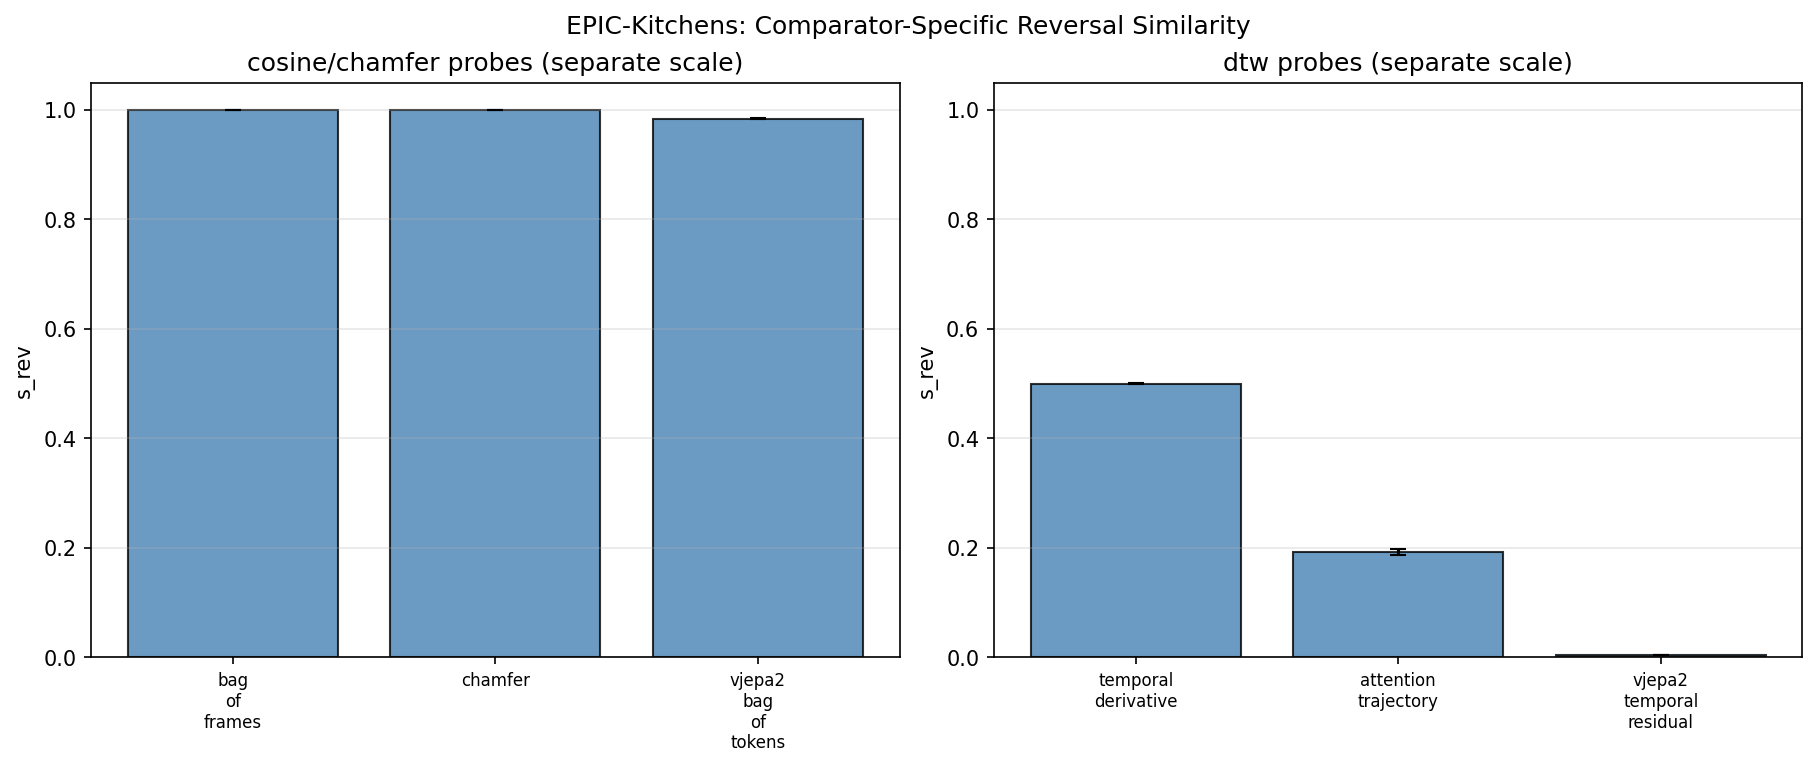
\includegraphics[width=0.9\textwidth]{../figures/epic_temporal_order_sensitivity.png}
    \caption{Order sensitivity ($s_\text{rev}$) across all embedding probes on EPIC-Kitchens (500 sequences). VLM vision towers are perfectly order-invariant when pooled ($s_\text{rev} \approx 1.0$), but per-frame sequences compared via DTW achieve perfect forward/reverse separation (balanced accuracy\,=\,1.0). LLM hidden states remain order-invariant regardless.}
    \label{fig:epic_sensitivity}
\end{figure}

\section{Full Scene Matching Results}
\label{sec:scene_matching}

We evaluated models across three scene-matching datasets: VCDB~\cite{vcdb} (copy detection), Nymeria~\cite{nymeria} (egocentric activity discrimination), and MUVR~\cite{muvr} (untrimmed multi-modal news/dance retrieval).

\begin{table}[h]
\centering
\caption{Retrieval AP driven by scene appearance / visual noise. VCDB: 528 videos, 5{,}585 positive pairs; Nymeria: 100 egocentric sessions, 8{,}780 segments; MUVR News: 9{,}958 videos, 74 topics.}
\begin{tabular}{lccc}
\toprule
\textbf{Method} & \textbf{VCDB} & \textbf{Nymeria} & \textbf{MUVR (News)} \\
\midrule
\textbf{BoF (DINOv3)} & 0.979 & \textbf{0.485} & 0.731 \\
\textbf{Chamfer matching (DINOv3)} & \textbf{0.989} & 0.482 & \textbf{0.746} \\
Temporal Residual (V-JEPA 2) & 0.698 & 0.279 & 0.505 \\
Attention Trajectory (DINOv3) & 0.700 & 0.217 & 0.466 \\
\bottomrule
\end{tabular}
\end{table}

BoF and Chamfer matching consistently dominate. On Nymeria, the 100-session scale confirms that scene appearance remains the strongest signal even with high intra-class variability (AP\,$\approx$\,0.48). On MUVR News, matching events share visual backgrounds (e.g., news desks), favoring semantic pooling. Attention Trajectories fail because egocentric gaze and semantic pacing vary unpredictably, introducing severe intra-class noise.

\section{Preliminary: Qwen3-VL on VCDB}
\label{sec:qwen_vcdb}

We first tested whether Video-LLMs can detect temporal reversal. Using Qwen3-VL~\cite{qwen3vl}, we presented forward and reversed versions of 49 VCDB videos and asked for temporal direction classification (3 trials each).

\begin{table}[h]
\centering
\caption{Qwen3-VL reversal detection on VCDB. Chance = 50\%.}
\begin{tabular}{llccc}
\toprule
\textbf{Model} & \textbf{Dataset (N)} & \textbf{Fwd Acc.} & \textbf{Rev Acc.} & \textbf{Overall} \\
\midrule
Qwen3-VL-4B-Instruct & Single clip (1) & 100\% & 0\% & 50.0\% \\
Qwen3-VL-30B-A3B & VCDB subset (49) & 83.0\% & 28.6\% & 55.8\% \\
\bottomrule
\end{tabular}
\end{table}

The 30B model achieves 55.8\%, near chance. The slight improvement is driven by a content-dependent FORWARD bias (83\% forward, 28.6\% reverse), not temporal understanding. This motivated the systematic multi-VLM evaluation on EPIC-Kitchens (Section~\ref{sec:vlm_generative}).

\section{VLM Temporal Integrity Probe}
\label{sec:integrity_probe}

Separately from forward/reverse classification, we asked VLMs to judge whether a video's temporal structure is ``INTACT'' or ``TAMPERED,'' on forward, reversed, and chunk-scrambled ($K\!=\!4, 16$) versions of EPIC-Kitchens sequences.

\begin{table}[h]
\centering
\caption{Temporal integrity probe on EPIC-Kitchens (500 sequences): fraction judged TAMPERED. LLaVA excluded from aggregate due to constant-output degeneracy.}
\begin{tabular}{lcccc}
\toprule
\textbf{Model} & \textbf{Forward} & \textbf{Reversed} & \textbf{Scramble $K\!=\!4$} & \textbf{Scramble $K\!=\!16$} \\
\midrule
Qwen3-VL-8B & 0.112 & 0.870 & 0.668 & 0.660 \\
Gemma-4-31B & 0.150 & 0.840 & 0.202 & 0.220 \\
LLaVA-Video-7B$^\dagger$ & 1.000 & 1.000 & 1.000 & 1.000 \\
\bottomrule
\end{tabular}
\begin{flushleft}
\small $^\dagger$LLaVA produces constant ``TAMPERED'' regardless of input (text-only baseline confirms). Excluded from integrity analysis.
\end{flushleft}
\end{table}

Qwen and Gemma correctly identify forward videos as INTACT ($\sim$85--89\%) and both flag reversed videos as TAMPERED (Qwen~87\%, Gemma~84\%). Scramble detection diverges: Qwen flags 67\% of scrambled videos ($K\!=\!4$) as TAMPERED while Gemma flags only 20\%, suggesting the two models rely on different heuristics. Cross-transform consistency is very low (3.8--8.2\%).

\section{VLM Prompt Sensitivity and Text-Only Baselines}
\label{sec:prompt_details}

Answers on forward/reverse classification are dominated by prompt phrasing, not visual content. Gemma-4 exhibits opposite biases across prompts: prompt~0 yields 87\% reverse bias; prompt~2 yields 73\% forward bias. LLaVA-Video answers ``FORWARD'' for prompts~0--1 ($>$98\%) but ``REVERSE'' for prompt~2 (83\%). Text-only baselines confirm these are prior biases; Qwen3 shows no text-only bias but still performs at chance with video.

LLaVA-Video produces constant ``TAMPERED'' regardless of input (text-only baseline confirms prior bias). We exclude it from aggregate integrity statistics in Appendix~\ref{sec:integrity_probe}.

\section{HDD Leakage Analysis}
\label{sec:hdd_leakage}

Since V-JEPA~2 temporal residuals achieve AP\,=\,0.956 on Honda HDD, well above the next-best method (BoT, AP\,=\,0.825), we verify that no metadata leakage inflates this result.

\textbf{Feature inputs.} All six methods receive \emph{only} decoded video frames. GPS is used exclusively for DBSCAN clustering; timestamps select the frame window ($\pm$3\,s) and are discarded before extraction.

\textbf{Segment duration.} Maneuver segments span 7.0--46.0\,s (mean 10.1\,s). Left and right turns have similar duration distributions (left: $10.3 \pm 3.8$\,s; right: $9.9 \pm 3.6$\,s), ruling out duration as a shortcut. V-JEPA~2 pads all segments to 64 frames, eliminating length signal.

\textbf{Cluster composition.} Only ``mixed'' clusters containing both turn directions are used. Within each, all $\binom{n}{2}$ pairs are evaluated, ensuring models must distinguish maneuver type at the same location.

\textbf{Cross-session control.} To rule out session adjacency confounds, we re-evaluate excluding same-session pairs (91.4\% of pairs are already cross-session). AP is unchanged: V-JEPA~2 temporal residual 0.957 (cross-session) vs.\ 0.956 (all pairs); BoF 0.536 vs.\ 0.530. This confirms results are not inflated by within-session visual correlations.

\textbf{Mechanistic explanation.} The context sweep (Section~\ref{sec:context_sweep}) shows temporal residual AP degrades monotonically as context narrows, consistent with genuine temporal processing. BoF methods remain near chance across all windows.

\textbf{Motion proxy check.} To rule out trivial motion magnitude as a shortcut, we compute mean pixel difference between consecutive frames for each segment and correlate pairwise proxy similarity with V-JEPA~2 residual similarity across all 97{,}731 pairs. Spearman $r = 0.051$; the motion proxy itself achieves only AP\,=\,0.474 (below chance). Residuals capture motion \emph{structure}, not intensity.

\section{VCDB Negative-Sampling Sensitivity}
\label{sec:neg_sampling}

Our primary VCDB evaluation uses 1:1 positive-to-negative sampling (5{,}585 pairs each). The full dataset contains $\binom{528}{2} \approx 139$K possible pairs. We re-evaluate at three ratios to verify robustness (Table~\ref{tab:neg_sensitivity}).

\begin{table}[h]
\centering
\caption{VCDB AP across negative-sampling ratios. \emph{Rank order and relative gaps are stable across all settings.} All-pairs uses the full $\binom{528}{2}$ set (requiring ${\sim}140$K DTW comparisons).}
\label{tab:neg_sensitivity}
\begin{tabular}{lccc}
\toprule
\textbf{Method} & \textbf{1:1} & \textbf{1:5} & \textbf{All pairs} \\
\midrule
DINOv3 Chamfer           & 0.989 & 0.949 & 0.845 \\
DINOv3 BoF               & 0.979 & 0.929 & 0.829 \\
DINOv3 Temporal Deriv.   & 0.713 & 0.424 & 0.228 \\
DINOv3 Attn.\ Trajectory & 0.700 & 0.408 & 0.225 \\
\bottomrule
\end{tabular}
\begin{flushleft}
\small Rank order (Chamfer $>$ BoF $>$ Temporal Deriv.\ $>$ Attn.\ Trajectory) is preserved across all ratios. AP decreases with more negatives as expected; AUC remains stable (e.g.\ Chamfer AUC: 0.990, 0.989, 0.989). The 1:1 temporal derivative AP (0.713) differs from Table~\ref{tab:summary} (0.775) because this analysis uses independently sampled negatives with a different seed; rank order is unaffected.
\end{flushleft}
\end{table}

\section{Bootstrap Confidence Intervals}
\label{sec:bootstrap_cis}

Table~\ref{tab:bootstrap} reports 95\% bootstrap confidence intervals (2{,}000 resamples, percentile method, seed\,=\,42) for the headline AP values from Tables~1--3. Degenerate bootstrap samples (all-positive or all-negative) fall back to the point estimate.

\begin{table}[h]
\centering
\caption{95\% bootstrap CIs for AP across all benchmarks. ``Width'' is CI\textsubscript{high}\,$-$\,CI\textsubscript{low}. VCDB and HDD CIs are narrow ($<$0.02); nuScenes, Nymeria, and MUVR CIs are wider due to smaller evaluation sets.}
\label{tab:bootstrap}
\begin{tabular}{llccc}
\toprule
\textbf{Benchmark} & \textbf{Method} & \textbf{AP} & \textbf{95\% CI} & \textbf{Width} \\
\midrule
\multirow{4}{*}{VCDB}
 & DINOv3 Chamfer           & 0.989 & [0.987, 0.991] & 0.004 \\
 & DINOv3 BoF               & 0.979 & [0.976, 0.981] & 0.005 \\
 & DINOv3 Temporal Deriv.   & 0.775 & [0.765, 0.784] & 0.019 \\
 & DINOv3 Attn.\ Trajectory & 0.700 & [0.689, 0.711] & 0.022 \\
 & V-JEPA 2 BoT             & 0.838 & [0.829, 0.846] & 0.017 \\
 & V-JEPA 2 Temporal Res.   & 0.698 & [0.687, 0.709] & 0.022 \\
\midrule
\multirow{6}{*}{HDD}
 & V-JEPA 2 Temporal Res.   & 0.956 & [0.955, 0.958] & 0.003 \\
 & V-JEPA 2 BoT             & 0.825 & [0.821, 0.828] & 0.007 \\
 & DINOv3 Chamfer           & 0.559 & [0.555, 0.564] & 0.009 \\
 & DINOv3 BoF               & 0.529 & [0.525, 0.534] & 0.009 \\
 & DINOv3 Attn.\ Trajectory & 0.507 & [0.502, 0.512] & 0.010 \\
 & DINOv3 Temporal Deriv.   & 0.498 & [0.494, 0.503] & 0.009 \\
\midrule
\multirow{7}{*}{nuScenes}
 & V-JEPA 2 Encoder-Seq DTW & 0.867 & [0.842, 0.890] & 0.048 \\
 & V-JEPA 2 Temporal Res.   & 0.815 & [0.785, 0.844] & 0.059 \\
 & V-JEPA 2 BoT             & 0.791 & [0.761, 0.820] & 0.059 \\
 & DINOv3 Temporal Deriv.   & 0.623 & [0.580, 0.665] & 0.085 \\
 & DINOv3 BoF               & 0.613 & [0.570, 0.658] & 0.088 \\
 & DINOv3 Chamfer           & 0.612 & [0.570, 0.659] & 0.089 \\
 & DINOv3 Attn.\ Trajectory & 0.584 & [0.540, 0.634] & 0.094 \\
\midrule
\multirow{6}{*}{Nymeria}
 & DINOv3 BoF               & 0.485 & [0.482, 0.489] & 0.007 \\
 & DINOv3 Chamfer           & 0.482 & [0.478, 0.485] & 0.007 \\
 & DINOv3 Temporal Deriv.   & 0.274 & [0.271, 0.277] & 0.006 \\
 & DINOv3 Attn.\ Trajectory & 0.217 & [0.215, 0.219] & 0.004 \\
 & V-JEPA 2 BoT             & 0.420 & [0.417, 0.424] & 0.007 \\
 & V-JEPA 2 Temporal Res.   & 0.278 & [0.276, 0.281] & 0.005 \\
\midrule
\multirow{6}{*}{MUVR News}
 & DINOv3 BoF               & 0.731 & [0.724, 0.740] & 0.016 \\
 & DINOv3 Chamfer           & 0.745 & [0.738, 0.754] & 0.016 \\
 & DINOv3 Temporal Deriv.   & 0.476 & [0.468, 0.485] & 0.017 \\
 & DINOv3 Attn.\ Trajectory & 0.466 & [0.458, 0.475] & 0.017 \\
 & V-JEPA 2 BoT             & 0.597 & [0.587, 0.605] & 0.018 \\
 & V-JEPA 2 Temporal Res.   & 0.505 & [0.496, 0.514] & 0.018 \\
\bottomrule
\end{tabular}
\begin{flushleft}
\small VCDB and HDD CIs are narrow ($<$0.025) under pair-level resampling. nuScenes CIs are wider (0.06--0.09) due to the smaller evaluation set (950 pairs), but rank order remains unambiguous. Nymeria CIs are very tight ($<$0.01) despite the scene-retrieval setting (394{,}210 pairs). MUVR News CIs (0.016--0.018) reflect the moderate evaluation set (27{,}453 pairs). \textbf{Note:} pair-level resampling underestimates CI width because pairs within a GPS cluster share clips. A cluster-level block bootstrap (resampling clusters with replacement) produces CIs 7--32$\times$ wider on HDD: e.g., V-JEPA~2 temporal residual widens from [0.955,\,0.958] to [0.890,\,0.978]. Rank order is preserved; the pair-level CIs should be read as lower bounds on uncertainty.
\end{flushleft}
\end{table}

\section{HDD Qualitative Analysis}
\label{sec:hdd_qualitative}

To complement the quantitative maneuver discrimination results, we present qualitative evidence that V-JEPA~2 temporal residuals capture genuine motion dynamics rather than exploiting a visual shortcut.

\textbf{Nearest-neighbor examples.} For three representative intersection clusters, the top-3 neighbors by temporal residual similarity retrieve the same maneuver type despite identical backgrounds; errors occur when both turns share similar speeds through the same intersection phase.

\textbf{Background similarity statistics.} Within each GPS cluster, all segments share the same intersection. BoF cosine similarity for all $\binom{n}{2}$ pairs per cluster: mean $0.63 \pm 0.18$ (same-direction: $0.63 \pm 0.18$; cross-direction: $0.60 \pm 0.16$; gap = $0.029$), confirming appearance is non-discriminative. V-JEPA~2 temporal residual similarity aligns with maneuver labels (same: $0.008 \pm 0.006$; cross: $0.003 \pm 0.001$). Figure~\ref{fig:hdd_qualitative} shows the score distributions.

\begin{figure}[h]
\centering
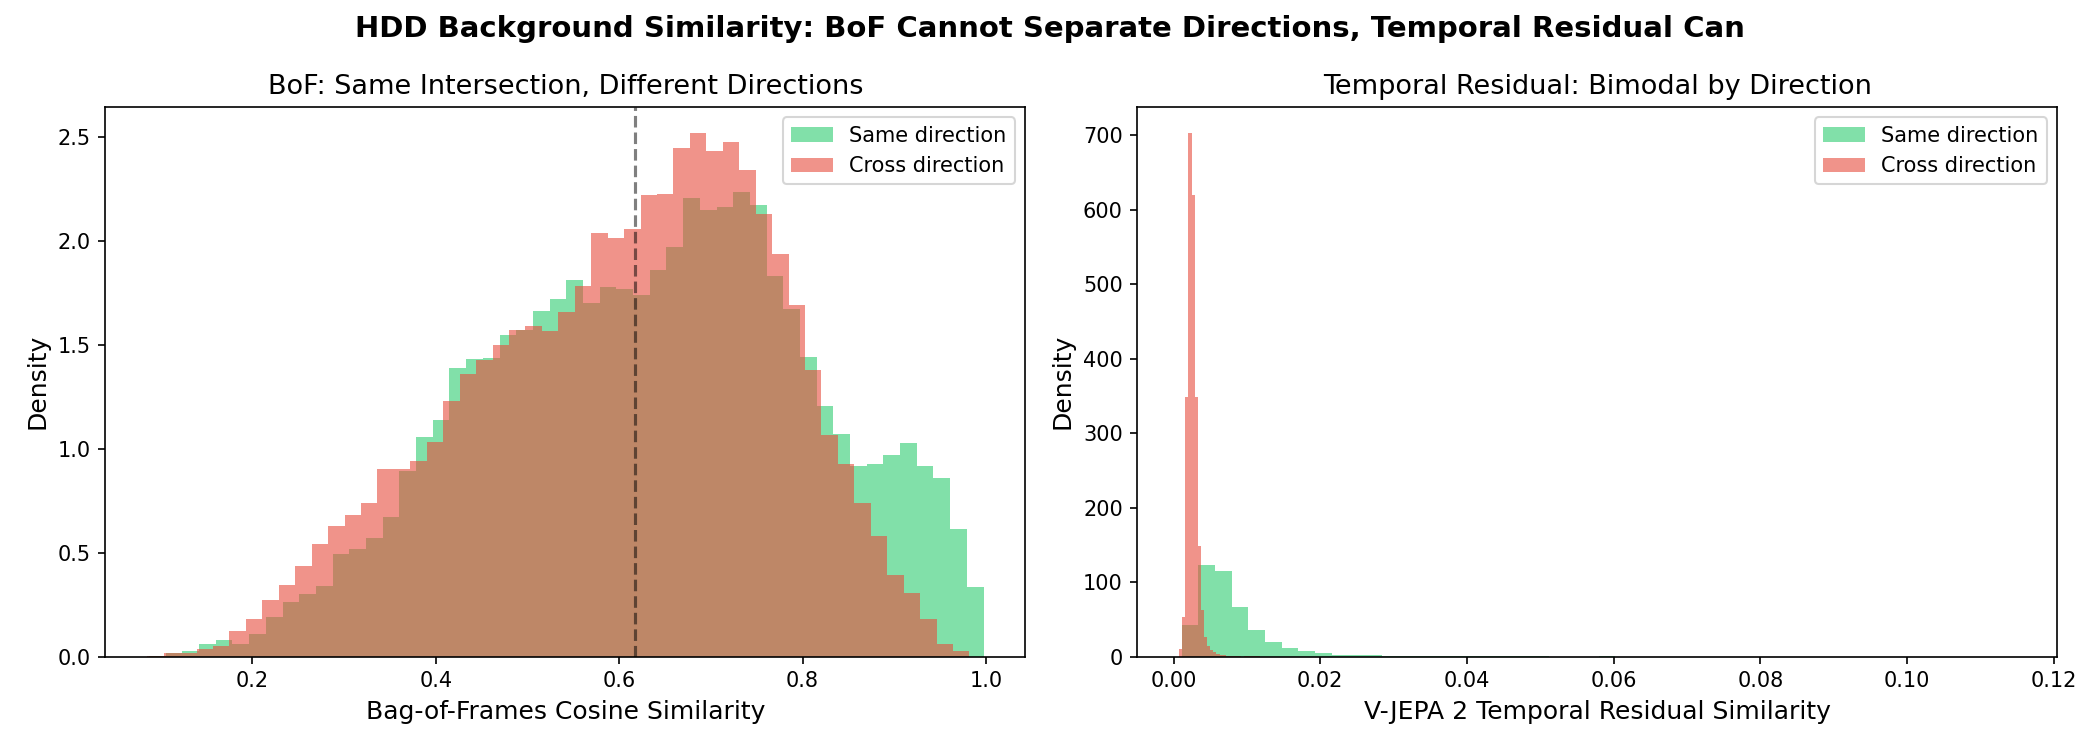
\includegraphics[width=\linewidth]{../figures/hdd_qualitative_distributions.png}
\caption{Pairwise similarity distributions on HDD intersection clusters. BoF similarities overlap heavily regardless of maneuver match, while V-JEPA~2 temporal residual scores separate same- vs.\ cross-direction pairs.}
\label{fig:hdd_qualitative}
\end{figure}

\section{nuScenes Cross-Dataset Visualization}
\label{sec:nuscenes_figure}

\begin{figure}[h]
    \centering
    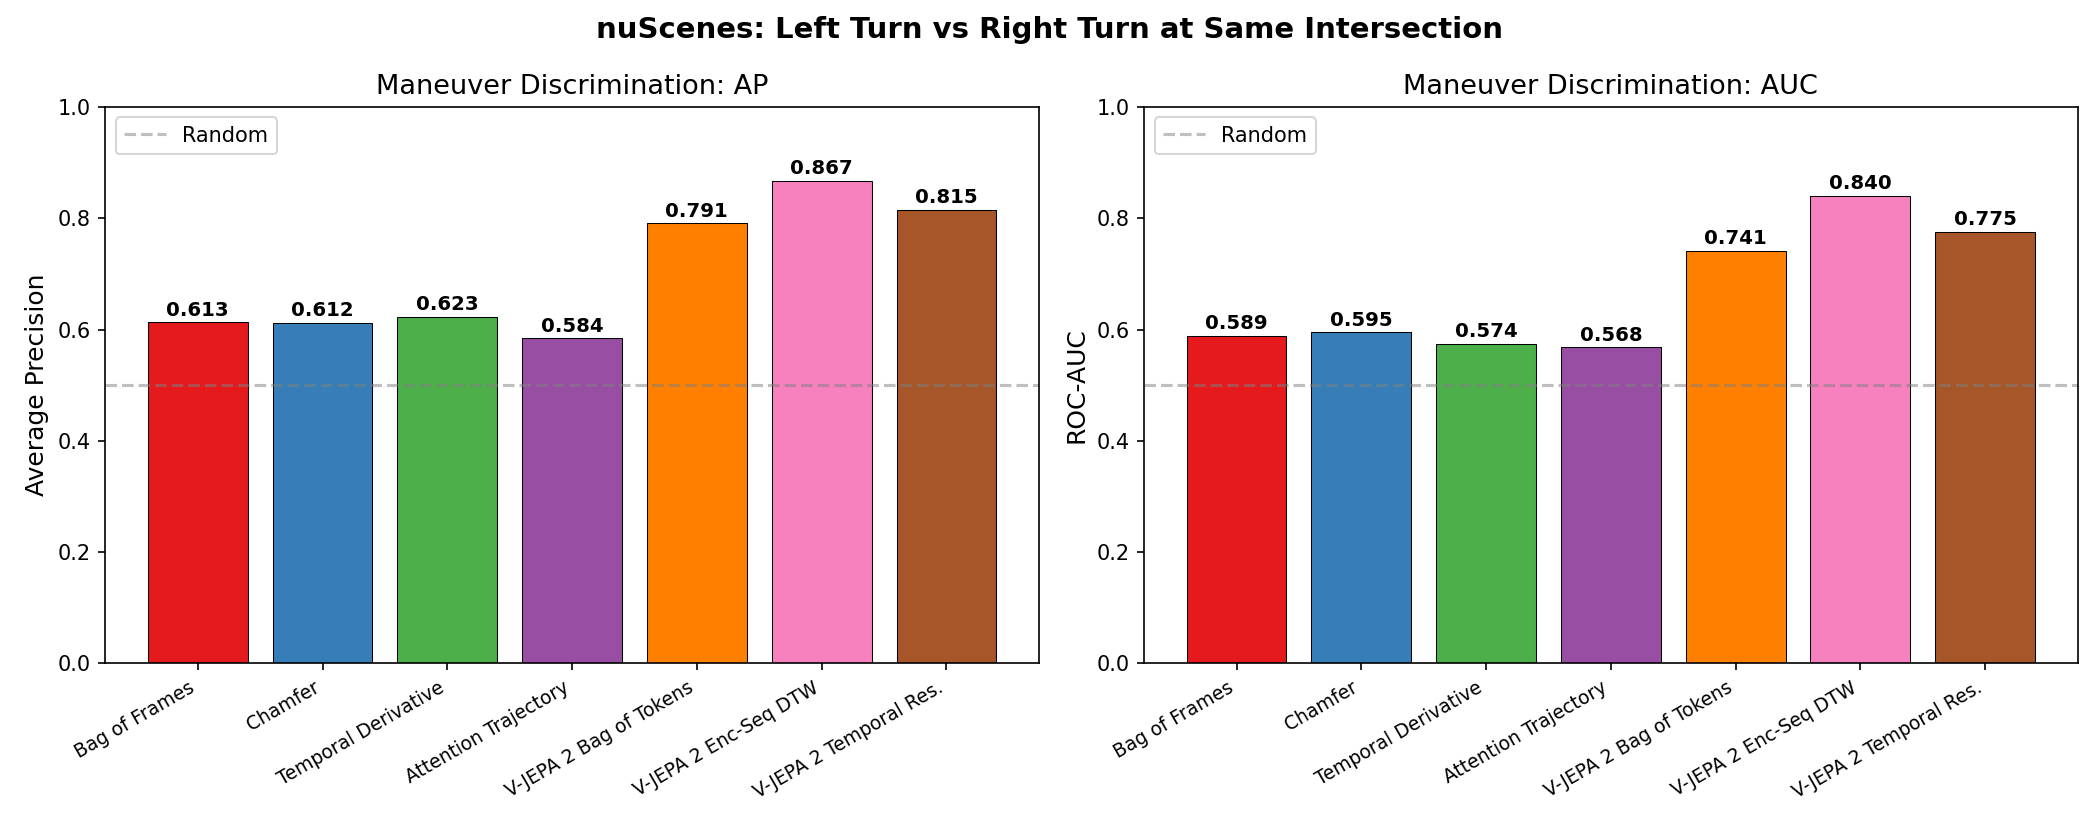
\includegraphics[width=0.9\textwidth]{../figures/nuscenes_maneuver_discrimination.png}
    \caption{nuScenes cross-dataset validation (264 segments, 950 pairs, 50 intersection clusters). V-JEPA~2 encoder-sequence DTW (AP\,=\,0.867) is the strongest method; the comparator change alone surpasses the temporal residual (AP\,=\,0.815).}
    \label{fig:nuscenes_maneuver}
\end{figure}

\section{LLM Hidden-State Probe: Vision-Token-Only Analysis}
\label{sec:vision_token_probe}

A potential objection to our LLM hidden-state probe is that mean-pooling over \emph{all} tokens reintroduces symmetric aggregation. To address this, we extract LLM hidden states restricted to \emph{vision-token positions only}. Three variants:

\begin{enumerate}
    \item \textbf{Vision-only mean pool}: Mean-pool LLM hidden states at vision-token positions only. Compare via cosine similarity.
    \item \textbf{Vision-only per-frame sequence}: Group vision-token hidden states by their source frame, pool per frame to obtain a $(T, D)$ sequence. Compare via temporal derivative DTW.
    \item \textbf{BOS/first token}: Use the first token's hidden state (BOS or system token) as a summary representation. Compare via cosine similarity.
\end{enumerate}

\begin{table}[h]
\centering
\caption{$s_\text{rev}$ for vision-token-only LLM hidden-state probes (EPIC-Kitchens, 500 sequences). If vision-only pooling recovers temporal signal, we expect $s_\text{rev} \ll 1.0$; if order-invariance persists, the conclusion from Section~\ref{sec:vlm_embedding} is strengthened.}
\label{tab:vision_token_probe}
\begin{tabular}{lccc}
\toprule
\textbf{Model} & \textbf{Vision-only pool} & \textbf{Vision-only seq DTW} & \textbf{BOS token} \\
\midrule
Qwen3-VL-8B    & 0.998 [0.998, 0.998] & \textbf{0.542} [0.540, 0.544] & 0.996 \\
Gemma-4-31B    & 1.000 [1.000, 1.000]$^\dagger$ & \textbf{0.509} [0.509, 0.509] & 1.000 \\
LLaVA-Video-7B & 0.999 [0.998, 0.999] & \textbf{0.517} [0.516, 0.518] & 1.000$^\dagger$ \\
\bottomrule
\end{tabular}
\begin{flushleft}
\small Vision-only mean pooling remains $s_\text{rev} \approx 1.0$ across all models, confirming that symmetric aggregation, not the LLM backbone, erases temporal signal. The per-frame sequence probe yields low $s_\text{rev}$ (balanced accuracy\,=\,1.0), showing that LLM hidden states preserve per-position order information that pooling discards. BOS tokens are order-invariant, indicating the model's summary position captures no temporal signal. $^\dagger$Raw values $>$1.0 from f32 precision; clamped to 1.000.
\end{flushleft}
\end{table}

\section{Scramble Gradient Data}
\label{sec:scramble_data}

\begin{table}[h]
\centering
\caption{AP across scramble levels $K$ on VCDB (527 of 528 videos; one decode failure). $K\!=\!1$ is the unscrambled baseline. Order-invariant methods show constant AP; sequence-aware methods show overall degradation (multi-seed analysis: $\sigma \leq 0.007$; Figure~\ref{fig:scramble_multiseed}).}
\resizebox{\textwidth}{!}{%
\begin{tabular}{lcccccccc}
\toprule
\textbf{Method} & $K\!=\!1$ & $K\!=\!2$ & $K\!=\!3$ & $K\!=\!4$ & $K\!=\!6$ & $K\!=\!8$ & $K\!=\!12$ & $K\!=\!16$ \\
\midrule
BoF (DINOv3) & 0.979 & 0.979 & 0.979 & 0.979 & 0.979 & 0.979 & 0.979 & 0.979 \\
Chamfer (DINOv3) & 0.989 & 0.989 & 0.989 & 0.989 & 0.989 & 0.989 & 0.989 & 0.989 \\
V-JEPA 2 BoT & 0.838 & 0.838 & 0.838 & 0.838 & 0.838 & 0.838 & 0.838 & 0.838 \\
Temporal Derivative (DINOv3) & 0.775 & 0.735 & 0.733 & 0.734 & 0.724 & 0.731 & 0.729 & 0.722 \\
V-JEPA 2 Temporal Residual & 0.698 & 0.612 & 0.633 & 0.609 & 0.601 & 0.618 & 0.609 & 0.639 \\
\textbf{Attention Trajectory (DINOv3)} & 0.700 & 0.650 & 0.631 & 0.619 & 0.598 & 0.596 & 0.585 & 0.572 \\
\bottomrule
\end{tabular}
}
\end{table}

V-JEPA~2 residuals show non-monotonic degradation (e.g.\ $K\!=\!3$ higher than $K\!=\!2$), likely due to boundary effects where the spatiotemporal prediction window crosses chunk boundaries. A multi-seed analysis (10 independent shuffle seeds per $K$) shows that order-invariant methods have zero variance ($\sigma = 0.000$), while temporal methods show small but real variation ($\sigma \leq 0.007$) that does not affect method ranking (Figure~\ref{fig:scramble_multiseed}). Because the main scramble gradient shuffles \emph{extracted} embeddings, it tests whether the comparator (DTW) is sensitive to temporal order, not whether V-JEPA's encoder responds differently to scrambled input. A raw-frame scramble (re-running V-JEPA~2 on chunk-shuffled video) produces clean monotonic degradation: residual AP drops from 0.705 at $K\!=\!1$ to 0.652 at $K\!=\!16$, while BoT remains flat at 0.839. The encoder does produce different residuals from temporally disrupted input.

\begin{figure}[h]
    \centering
    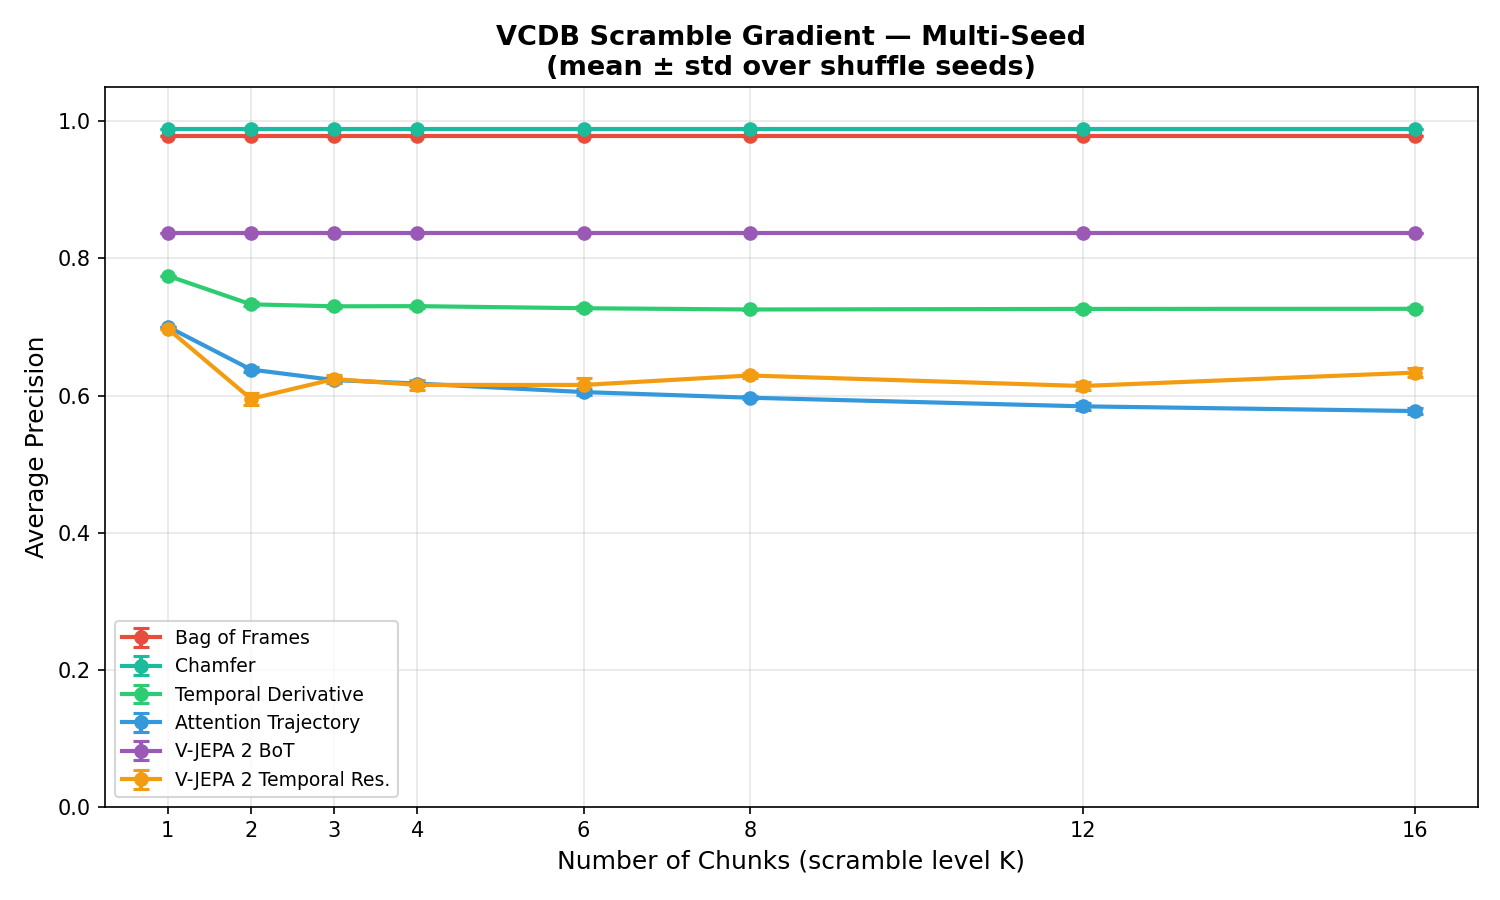
\includegraphics[width=0.9\textwidth]{../figures/vcdb_scramble_multiseed.png}
    \caption{Multi-seed scramble gradient on VCDB (10 seeds per $K$, mean $\pm$ std shaded). Order-invariant methods (BoF, Chamfer, V-JEPA~2 BoT) have zero variance. Temporal methods show small variance ($\sigma \leq 0.007$) that does not change the ranking.}
    \label{fig:scramble_multiseed}
\end{figure}

\section{Linear Probe on LLM Hidden States}
\label{sec:linear_probe}

The $s_\text{rev}$ analysis (Section~\ref{sec:vlm_embedding}) shows that mean-pooled LLM hidden states are order-invariant. A natural follow-up: is temporal signal present in the per-position hidden states but lost to symmetric aggregation? If so, a learned classifier should recover it.

We extract last-layer hidden states from all three VLMs for 200 EPIC-Kitchens sequences (forward and reverse), yielding 400 samples per model. We train $\ell_2$-regularized logistic regression (5-fold GroupKFold CV, fwd/rev pairs kept together, $C \in \{0.01, 0.1, 1, 10, 100\}$) on seven readout strategies:

\begin{itemize}
    \item \textbf{mean}: mean over all positions (replicates $s_\text{rev}$ finding)
    \item \textbf{max}: element-wise max over all positions
    \item \textbf{first} / \textbf{last}: single position (BOS or final token)
    \item \textbf{concat\_first\_last}: concatenation of first and last positions
    \item \textbf{vision\_mean}: mean restricted to vision-token positions
    \item \textbf{vision\_concat\_fl}: first and last vision-token positions
\end{itemize}

\begin{table}[h]
\centering
\caption{Probe accuracy (GroupKFold CV, fwd/rev pairs kept together) for forward vs.\ reverse classification from LLM hidden states. Linear = logistic regression (best across $C \in \{0.01, 0.1, 1, 10, 100\}$); MLP = 2-layer, 256 hidden units, ReLU. Chance = 0.500. No configuration exceeds chance.}
\label{tab:linear_probe}
\resizebox{\textwidth}{!}{%
\begin{tabular}{lcccccc}
\toprule
& \multicolumn{2}{c}{\textbf{Gemma-4 31B}} & \multicolumn{2}{c}{\textbf{LLaVA-Video 7B}} & \multicolumn{2}{c}{\textbf{Qwen3-VL 8B}} \\
\cmidrule(lr){2-3} \cmidrule(lr){4-5} \cmidrule(lr){6-7}
\textbf{Pooling} & \textbf{Linear} & \textbf{MLP} & \textbf{Linear} & \textbf{MLP} & \textbf{Linear} & \textbf{MLP} \\
\midrule
mean                & 0.512 & 0.552 & 0.500 & 0.505 & 0.537 & 0.510 \\
max                 & 0.532 & 0.458 & 0.470 & 0.490 & 0.528 & 0.502 \\
first               & 0.500 & 0.500 & 0.500 & 0.500 & 0.500 & 0.500 \\
last                & 0.510 & 0.507 & 0.515 & 0.495 & 0.550 & 0.512 \\
concat\_first\_last & 0.515 & 0.490 & 0.505 & 0.478 & 0.555 & 0.520 \\
vision\_mean        & 0.520 & 0.550 & 0.502 & 0.512 & 0.537 & 0.505 \\
vision\_concat\_fl  & 0.528 & 0.500 & 0.495 & 0.467 & 0.515 & 0.535 \\
\bottomrule
\end{tabular}
}
\end{table}

Neither linear nor nonlinear probes recover temporal order from LLM hidden states. All 126 configurations (3 models $\times$ 7 pooling strategies $\times$ \{5 regularization strengths for linear, 1 for MLP\}) land between 0.458 and 0.560, within the range expected from chance on 400 samples. The ``first'' token gives exactly 0.500 under both probes, a sanity check that the pipeline is correct when the input is truly identical across conditions (BOS tokens do not change between forward and reverse).

Note that per-position LLM hidden states \emph{do} carry order signal when compared as a sequence via DTW ($s_\text{rev} \approx 0.51$--$0.54$; Table~\ref{tab:vision_token_probe}): order is encoded in the relative content across positions, but no fixed-dimensional reduction of the sequence retains it. This is the same pooling-destroys-order dynamic observed at the vision encoder level, replicated one layer deeper.

\section{Computational Costs}
\label{sec:computational_costs}

\begin{table}[h]
\centering
\caption{Per-video feature extraction and per-pair comparison costs on a single H200 GPU. $T$ = number of frames per clip.}
\begin{tabular}{lcc}
\toprule
\textbf{Method} & \textbf{Extraction (ms/video)} & \textbf{Comparison (ms/pair)} \\
\midrule
DINOv3 BoF ($T\!=\!30$) & ${\sim}120$ & $<$0.01 (cosine) \\
DINOv3 Chamfer ($T\!=\!30$) & ${\sim}120$ & ${\sim}0.3$ (frame matrix) \\
DINOv3 Attn.\ Trajectory ($T\!=\!30$) & ${\sim}150$ & ${\sim}1$ (DTW) \\
DINOv3 Temporal Deriv.\ ($T\!=\!30$) & ${\sim}120$ & ${\sim}1$ (DTW) \\
V-JEPA 2 BoT ($T\!=\!64$) & ${\sim}280$ & $<$0.01 (cosine) \\
V-JEPA 2 Temporal Res.\ ($T\!=\!64$) & ${\sim}560$ & ${\sim}1$ (DTW) \\
VLM vision pooled & ${\sim}800$--$2{,}500$ & $<$0.01 (cosine) \\
VLM LLM hidden state & ${\sim}1{,}500$--$5{,}000$ & $<$0.01 (cosine) \\
\bottomrule
\end{tabular}
\begin{flushleft}
\small V-JEPA~2 temporal residual requires both encoder and predictor forward passes, roughly doubling extraction cost vs.\ BoT. DTW comparison at $T \approx 30$ is ${\sim}1$\,ms; a top-100 reranking pass after FAISS~\cite{faiss} pre-filtering adds ${\sim}100$\,ms total, making two-stage retrieval practical for production workloads.
\end{flushleft}
\end{table}

\section{Dataset and Model Licenses}
\label{sec:licenses}

All experiments use publicly available datasets and pretrained models. Table~\ref{tab:licenses} lists the governing license for each asset. Use is restricted to non-commercial research, consistent with the most restrictive license among the assets combined in any given experiment. No new datasets or model weights are released by this paper.

\begin{table}[h]
\centering
\small
\caption{Licenses for datasets and pretrained model weights used in this work. Verbatim license text is available from each asset's canonical distribution channel; see \texttt{REPRODUCIBILITY.md} for HuggingFace IDs and download URLs.}
\label{tab:licenses}
\begin{tabular}{lll}
\toprule
\textbf{Asset} & \textbf{License} & \textbf{Distribution} \\
\midrule
\multicolumn{3}{l}{\emph{Datasets}} \\
VCDB~\cite{vcdb}                      & Research-only; no warranty (Fudan Univ.)    & Project page \\
Honda HDD~\cite{honda_hdd}            & HRI-USA Data Use Agreement (non-commercial) & HRI-USA \\
nuScenes~\cite{nuscenes}              & CC BY-NC-SA 4.0                             & nuscenes.org \\
EPIC-Kitchens-100~\cite{epickitchens} & CC BY-NC 4.0                                & epic-kitchens.github.io \\
Nymeria~\cite{nymeria}                & CC BY-NC 4.0                                & facebookresearch GH \\
MUVR~\cite{muvr}                      & Research-only (authors' terms)              & Authors' release \\
\midrule
\multicolumn{3}{l}{\emph{Pretrained model weights}} \\
DINOv3~\cite{dinov3}                  & Meta FAIR non-commercial                    & HuggingFace \\
V-JEPA~2~\cite{vjepa2}                & CC BY-NC 4.0                                & HuggingFace \\
ViCLIP / InternVid~\cite{viclip}      & Apache 2.0 (code); CC BY-NC 4.0 (weights)   & OpenGVLab \\
X-CLIP~\cite{xclip}                   & MIT                                         & microsoft/VideoX \\
Qwen3-VL-8B~\cite{qwen3vl}            & Apache 2.0                                  & HuggingFace \\
Gemma~4~\cite{gemma4}                 & Gemma Terms of Use                          & HuggingFace \\
LLaVA-Video~\cite{llavavideo}         & Apache 2.0 (code); Llama-2 terms (weights)  & HuggingFace \\
RAFT (optical flow)                   & BSD-3-Clause                                & princeton-vl/RAFT \\
\bottomrule
\end{tabular}
\end{table}

Honda HDD access required a signed Data Use Agreement with HRI-USA; nuScenes required account registration at nuscenes.org; other datasets are downloadable under their respective non-commercial licenses. All assets were used for non-commercial research evaluation only.

\end{document}
